\documentclass[main.tex]{subfiles}
Resources for this section are my own lecture notes from Professor Corwin's Fall 2019 Analysis \& Probability I course and \textit{Probability Theory and Examples, 5th ed.} By Rick Durrett.

\subsection{Basic Measure Theory}
\subsubsection{Definition of a Measure and Basic Properties}
\begin{definition}[$\sigma$-algebra]
Let $\om$ be a set. We say $\cF \subset 2^{\om}$ is a $\sigma$-algebra if,
\begin{enumerate}
    \item $\om \in \cF$
    \item If $A \in \cF$, then $A^c \in \cF$
    \item For every countable collection $\{A_i\} \subset \cF$, $\bigcup A_i \subset \cF$
\end{enumerate}
Note that given 2 we could equivalently require that 1 read $\phi \in \cF$ and that 3 read that $\cF$ is closed to countable intersections.
\end{definition}

\begin{definition}[Measurable Space]
A pair $(\om, \cF)$ is called a measurable space.
\end{definition}

\begin{definition}[Measure and Probability Measure]
A measure $\mu$ on $(\om, \cF)$ is any countably additive, non-negative function, $\mu: \cF \to \R_{\geq 0}$ i.e. 
\begin{enumerate}
    \item $\mu(A) \geq \mu(\phi) = 0$
    \item $\mu(\bigcup_i A_i) \leq \sum_i \mu(A_i)$ with equality holding if the $A_i$ are disjoint (or if their intersections have measure 0)
\end{enumerate}
If $\mu(\om) = 1$, then we call $\mu$ a probability measure and often denote it by $\prob$.
\end{definition}

\begin{definition}
A measure $\mu$ on $(\om, \cF)$ is $\sigma$-finite if $\om = \bigcup_i A_i$ for $A_i \in \cF$ and $\mu(A_i) < \infty$ for all $i$.
\end{definition}
\begin{example}
All finite measures are $\sigma$-finite.
\end{example}
\begin{example}
The Lebesgue measure on $\R$ is $\sigma-finite$ with $A_i = [i, i+1]$ for $i \in \mathbb{Z}$
\end{example}

\begin{definition}[Measure Space and Probability Space]
We say that a triple $(\om, \cF, \mu)$ is a measure space. If $\mu$ is a probability measure, we call it a probability space.
\end{definition}

\begin{prop}
Given a probability space $(\om, \cF, \prob)$, the following hold,
\begin{enumerate}
    \item Monotonicity: if $A \subset B$, then $\prob(A) \leq \prob(B)$
    \item Continuity from above: if $A_1 \subset A_2 \subset ...$ such that $\bigcup_i A_i = A$ then $\prob(A_i) \to \prob (A)$
    \item Continuity from below: if $A_1 \supset A_2 \supset ...$ and $\bigcap_i A_i = A$ then $\prob(A_i) \to \prob(A)$
\end{enumerate}
\end{prop}

The proof of these properties follows pretty immediately from the definition.

\begin{prop}
For any collection $\cF \subset 2^{\om}$, there exists a unique $\sigma$-algebra $\sigma(\cF)$ such that,
\begin{enumerate}
    \item $\cF \subset \sigma(\cF)$
    \item for all $\sigma$-algebras $\mathcal{B}$ such that $\cF \subset \mathcal{B}$, $\sigma(\cF) \subset \mathcal{B}$
\end{enumerate}
\end{prop}
\begin{remark}
This construction requires the axiom of choice \textcolor{red}{why?}.
\end{remark}


\subsubsection{Carathéodory Extension Theorem}

We can use these minimally generated $\sigma$-algebras to define measures on spaces. First, we say that $\mathcal{A} \subset 2^{\om}$ is an algebra if it contains $\om$ and is closed to compliments and finite unions. 

\begin{theorem}[Carathéodory Extension Theorem]
Given a function,
\[\mu_0: \mathcal{A} \to \R_{\geq 0}\]
that is countably additive (known as a premeasure), there exists a measure,
\[\mu: \sigma(\mathcal{A}) \to \R_{\geq 0}\]
extending $\mu_0$, and if $\mu_0(\om) < \infty$ (known as being finite), then $\mu$ is unique.
\end{theorem}

\begin{proof}
We begin by defining an outer measure,$\mu^*: 2^{\om} \to \R \cup \{+\infty\}$ via the following formula:
\[\mu^*(A) = \inf\{\sum_i \mu (A_i)| A_i \in \cA, \bigcup_i A_i \supset A\}\]
Note that we can assume that the $A_i$ are disjoint by the countably additive assumption on $\mu$. We prove the following properties of this outer measure:
\begin{enumerate}
    \item Monotonicity
    \item Countably Subadditive
    \item $\mu^* = \mu$ on $\cA$
\end{enumerate}
Monotonicity is clear from the definition. For countably subadditve, we need to show,
$$\mu^*(\bigcup_i A_i) \leq \sum_i \mu^*(A_i)$$
Fix $\vep > 0$. There exists a $B_{i,j} \in \cA$ such that $\bigcup_j B_{i,j} \supset A_i$ and $\sum_j \mu(B_{i,j})\leq \mu^*(A_i) + \vep/2^i$ by definition of infimum. Then we have that,
\[\sum_i \mu^*(A_i) + \vep \geq \sum_{i,j} \mu(B_{i,j}) \geq \mu(\bigcup_{i,j}B_{i,j}) \geq \mu^*(\bigcup_i A_i)\]
where the second inequality follows from countable additivity on $\cA$ and the last follows by monotonicity.

To see that $\mu^* = \mu$ on $\cA$, note that by the countably additive property of $\mu$ the quantity $\sum_i \mu(A_i)$ for $A \subset \bigcup_i A_i$ is minimized when $A = \bigcup_i A_i$ and $\sum_i \mu(A_i) = \mu(\bigcup_i A_i) = \mu(A).$

We now define a subset $E \subset \om$ to be \textit{measurable} if for all other $A \subset \om$,
\[\mu^*(A) = \mu^*(A \cap E) + \mu^*(A \cap E^c)\]
Note that by the properties we've proven $\leq$ follows immediately, so we really only need to check $\geq$. We define $\cM$ to be the collection of all measurable sets. First we show that $\cM$ is an algebra.

\textcolor{red}{FINISH}

\end{proof}

The standard $\sigma$-algebra on $\R$ is the Borel $\sigma$-algebra $\cB$ defined as $\sigma(\mathcal{A})$ for $\mathcal{A} = \{(a_1,b_1] \cup .... \cup (a_k, b_k] | a_1 < b_1 < ... < a_k < b_k\}$. We define measures on $(\R, \cB)$ via distribution functions:

\begin{definition}
A Lebesgue-Steiljes distribution function $F: \R \to \R$ is a function that is non-decreasing and right continuous. Additionally, if $F(-\inf) = 0$ and $F(+\inf) = 1$, we call it a probability distribution function.
\end{definition}

We use these distribution functions to define measures on $\R$ by defining them on the generating algebra $\cA$ of $\cB$ to be,
\[\mu(\bigcup_{i = 1}^k (a_i, b_i]) = \sum_{i = 1}^{k} (F(b_i) - F(a_i))\]
In probability language, $F$ is the \textit{Cumulative Distribution Function} or CDF. When $F(x) = x$, we call the resulting measure the \textit{Lebesgue Measure} on $\R.$

\textcolor{red}{Include some comments about the space of measurable sets $\cM$ and how we define them via the axiom of choice}

\subsubsection{Measurable Functions and Random Variables}
We now move on to discussing the morphisms in the category of measurable spaces, measurable functions.
\begin{definition}[Measurable Function]
A function $X: (\om, \cF) \to (\om', \cF')$ is \textit{measurable} if for every $E \in \cF'$, $X^{-1}(E) \in \cF.$
\end{definition}

\begin{definition}[Random Variable and Random Vector]
If $(\om, \cF, \prob)$ is a probability space, and $X:(\om, \cF) \to (\R^d, \cB)$ is measurable, then $X$ is a random vector. In the case $d = 1$, $X$ is a random variable
\end{definition}


\begin{theorem}
If $\cA$ is a collection of subsets in $\om'$ such that $\sigma(\cA) = \cF'$, then $X$ is measurable if and only if for all $E \in \cA$, $X^{-1}(E) \in \cB$. That is, it is sufficient to check measurability on a generating set of your $\sigma$-algebra.
\end{theorem}
\begin{proof}
\textcolor{red}{Proof needed}
\end{proof}


\begin{definition}
For a function $X: (\om, \cF) \to (\om', \cF'),$ define $\sigma(X)$ to be the smallest $\sigma$-algebra on $\om$ such that $X: (\om, \sigma(X)) \to (\om', \cF')$ is measurable.
\end{definition}
\begin{remark}
Note that this construction also depends on $\cF$.
\end{remark}

\begin{prop}
A function $Y:(\om, \sigma(X)) \to (\om'', \cF'')$ is measurable if and only if $Y = f \circ X$ for some $f: (\om', \cF') \to (\om'', \cF'')$ measurable.
\end{prop}
\begin{proof}
\textcolor{red}{Proof needed QUESTION: IS THIS ONLY TRUE IN BOREL? Possible counter example: $\cF$ is the trivial $\sigma$-algebra}
\end{proof}

\begin{prop}
If $X, Y$ are measurable functions $(\om, \cF) \to (\R, \cB)$, then so are $X + Y$, $cX, XY,$ $\max(X,Y),$ $\min(X,Y),$ $\inf_n X_n,$ $sup_n X_n,$ $\liminf_x X_n,$ $\limsup_n X_n$. For $\{X_n\}_{n \geq 0}$, the set $\om = \{\omega \in \om| \lim(X_i(\omega)) \text{ exists}\}$ is a measurable set. \textcolor{red}{meaning it is in $\cF$?}
\end{prop}


\begin{theorem}[Lusin's]
If $f: \R \to \R$ is Borel measurable, then for all $\vep > 0$ there exists a continuous $g: \R \to \R$ such that the set $\{x|f(x) = g(x)\}$ is closed and the compliment has Lebesgue measure $\leq \vep$
\end{theorem}
\textcolor{red}{Check the statement of this because it was wonky in my notes}
In other words, any measurable function $f: \R \to \R$ can be closely approximated by a continuous function $g$. 

Now we consider how a measurable map pushes forward a measure on $(\om, \cF)$ to a measure on $(\om', \cF')$.

\begin{definition}[Distribution Function]
Let $(\om, \cF, \prob)$ be a probability space, $X$ a random variable. The distribution function of $X$, $F_X: \R \to [0,1]$ is defined by,
\[F_X(x) = \prob(\{\omega \in \om| X(\omega) \leq x
\})\]
Furthermore, this function defines a probability measure on $(\R, \cB)$.
\end{definition}
\begin{remark}
Random variables are \textit{not} defined by their distribution functions.
\end{remark}

\begin{prop}
All distribution functions have the following properties:
\begin{enumerate}
    \item Non-decreasing
    \item $\lim_{x \to +\infty} F(X) = 1, \lim_{x \to -\infty} F(X) = 0$
    \item Right continuous
    \item Left limits exist and are equal to $\prob(X < x)$ (we denote these limits as $F(x-)$)
    \item $F(x) - F(x-) = \prob(X = x)$
\end{enumerate}
\end{prop}

\subsubsection{Integration}
The goal of this section is to define integration with respect to a $\sigma$-finite measure $\mu$ on a measurable space $(\om, \cF)$. We construct $\int_{\om} f d\mu$ in 4 steps, at each stage we can verify the following properties:
\begin{enumerate}
    \item If $\varphi \geq 0$ almost everywhere, then $\int \varphi d\mu \geq 0$
    \item For all $a \in \R$, $\int a \varphi d\mu = a \int \varphi d \mu$. 
    \item $\int (\varphi + \psi) d\mu = \int \varphi d \mu + \int \psi d \mu$
    \item If $\varphi \leq \psi$ almost everywhere, $\int \varphi d \mu \leq \int \psi d \mu$
    \item $|\int \varphi d \mu| \leq \int |\varphi| d \mu$
\end{enumerate}

\paragraph{Step 1} For $\varphi$ a simple function $\varphi = \sum_{i = 1}^n a_i 1_{A_i}$, with $A_i$ disjoint measurable sets with $\mu(A_i) < \infty$, we define,
\[\int \varphi d \mu = \sum_{i = 1}^n a_i \mu(A_i)\]

\paragraph{Step 2} For $f$ bounded and $f = 0$ outside some $E$ such that $\mu(E) < \infty$, we define,
\[\int f d\mu = \sup_{\varphi \leq f} \int \varphi d \mu = \inf_{\psi \geq f} \int \psi d \mu\]
To prove that this equality is true, we can approximate our function $f$ from above and below by simple functions via the following sequences:
\[\psi_n = \sum_{k = -n}^n \frac{kM}{n}1_{f^{-1}([\frac{(k-1)M}{n}, \frac{kM}{n}])} \quad \quad \varphi_n = \sum_{k = -n}^n \frac{(k-1)M}{n}1_{f^{-1}([\frac{(k-1)M}{n}, \frac{kM}{n}])}\]
\begin{remark}
Note that, as opposed to Riemannian integration, this allows us to subdivide based on our range instead of our domain. This allows us to integrate more functions, for instance,
\[f(x) = \begin{cases}
1 & x \in \mathbb{Q}\\
0 & \text{else}
\end{cases}\]
can now be integrated on any bounded subset of $\R$.
\end{remark}

\paragraph{Step 3} For $f \geq 0$, we define,
\[\int f d\mu = \sup \{\int h d \mu| 0 \leq h \leq f, ||h||_{\infty} < \infty, \mu(\{x | h(x) \neq 0)\})<\infty\}\]

\paragraph{Step 4} Let $f$ be such that, as defined above, $\int|f| d \mu < \infty$ (we say $f$ is \textit{integrable}). Define,
\[f^-(x) = \begin{cases}
-f(x) & f(x) \leq 0\\
0 & \text{else}
\end{cases}
\quad \quad f^+(x) = \begin{cases}
f(x) & f(x) \geq 0\\
0 & \text{else}
\end{cases}\]
Then we define,
\[\int f d\mu = \int f^+ d\mu - \int f^- d\mu\]
\begin{remark}
For intuition as to why this is the correct notion of ``integrable", note that in the countable case we want to define the integral to be $\sum_{i \in \om} f(i) \mu(i)$, however if we do not have that this sum converges absolutely, that is, if $\sum_{i \in \om} |f(i)|\mu(i) = \infty$, then the sum $\sum_{i \in \om} f(i) \mu(i)$ can be rearranged to equal whatever value we want. This is clearly not a well defined notion of integration.
\end{remark}

The following is common notation for specific types of integrals,
\begin{enumerate}
    \item $(\R^d, \cB, \text{Lebesgue})$: $\int_A f(x) dx$
    \item $\om$ countable: $\int f d\mu = \sum_{i \in \om} f(i) \mu(i)$
    \item $(\R, \cB, \mu)$ with $\mu([a,b]) = G(b) - G(a)$: $\int f d\mu = \int f(x) dG$
\end{enumerate}

\begin{definition}[Expectation]
Let $\prob$ be a probability measure and $X$ a positive random variable. Then we define $\E[X] = \in X d\prob$. If $X$ is not necessarily $\geq 0$, we define $\E[X] = \int x^+ d\prob - \int X^- d\prob$ provided both $X^+$ and $X^-$ are integrable. A random variable $X$ is integrable if $\E[X] < \infty.$
\end{definition}

Now we can prove the first of the Borel-Cantelli lemmas:

\begin{definition}
    For $\{A_n\}_n$ a sequence of subsets in $\om$, 
    \[\limsup_{n \to \infty} A_n = \lim_{m \to \infty} \bigcup_{n = m}^{\infty} A_n = \limsup_{n \to \infty} 1_{A_n}\]
    (i.e. the set of all $\omega \in \om$ such that $\omega \in A_k$ for infinite $k$)
    \[\liminf_{n \to \infty} A_n = \lim_{m \to \infty} \bigcap_{n = m}^{\infty} A_n = \liminf_{n \to \infty} 1_{A_n}\]
    (i.e. the set of all elements $\omega \in \om$ such that $\omega \in A_k$ for all but finitely many $k$.
\end{definition}
    
\begin{lemma}[Borel-Cantelli Lemma (1)]
    If $\sum_{n = 1}^{\infty} \prob(A_n) < \infty$, then $\prob(\limsup_{n \to \infty} A_n) = 0$
\end{lemma}
    \begin{proof}
    Let $N(\omega) = \sum_{k = 1}^{\infty} 1_{A_k}(\omega)$. Then $\E[|N|] = \E[N] = \sum_{k = 1}^{\infty} \prob(A_k) < \infty$, therefore $N$ must be $< \infty$ almost surely.
\end{proof}
\begin{remark}
    The converse to this (that if the probabilities of the sets are not summable the $\limsup$ occurs with positive probability) is not true.
\end{remark}




\begin{prop}[Jensen's Inequality]
For $\varphi: \R \to \R$ convex, 
\[\varphi(\int f d \mu) \leq \int \varphi(f) d \mu\]
\end{prop}
\begin{proof}
    Let $L(x) = ax + b$ be a linear function such that $L(\int f d \mu) = \vp(\int f d \mu)$ and $L(x) \leq \vp(x)$ for all $x$ (such a function exists if $\vp$ is convex). Then we have,
    \[\int \vp(f) d \mu \geq \int af + b d\mu  = a \int f d\mu + b = L(\int f d\mu) = \vp(\int f d\mu)\]
\end{proof}


\begin{prop}[Holder's Inequality]
For $p,q \in (1,\infty)$ such that $\frac{1}{p} + \frac{1}{q} = 1$,
\[\int |fg| d \mu = ||fg||_1 \leq ||f||_p||g||_q\]
where $||f||_p = (\int |f|^pd\mu)^{1/p}$
\end{prop}
\begin{remark}
When $p = q = 2$, this is Cauchy-Schwartz inquality.
\end{remark}
\begin{proof}
    If $||f||_p$ or $||g||_p$ $= 0$, then $fg = 0$ almost everywhere. Therefore it is sufficient to prove the result when $||f||_p, ||g||_p> 0$. By deviding both sides by $||f||_p||g||_p$, we can assume that $||f||_p||g||_p = 1$. Fix $y \geq 0$ and for all $x \geq 0$, let,
    \[\vp(x) = x^p/p + y^q/q - xy\]
    Then we have that,
    \[\vp'(x) = x^{p-1} - y \quad \quad \vp''(x) = (p-1)x^{p-2}\]
    Therefore $x$ has a minimum at $x_0 = y^{1/(p-1)}$. Then we have that $q = p/(p-1)$, so $x_0^p = y^q$. Thus we have,
    \[\vp(x_0) = y^q(1/p + 1/q) - y^{1/(p-1)}y = 0\]
    Since $x_0$ was the minimum it follows that $xy \leq x^p/p + y^q/q$, so if we let $x = |f|, y = |g|$, we get,
    \[\int |fg|d\mu \leq \frac{1}{p} + \frac{1}{q} = 1 = ||f||_p||g||_p\]
\end{proof}

\begin{prop}[Markov's Inequality]
    Suppose $\vp: \R \to \R$ has $\vp \geq 0$. Let $A \in \cB$ and let $i_A = \inf\{\vp(a)|a\in A\}$. Then,
    \[i_A \prob(X \in A) \leq \E[\vp(X)1_{X \in A}] \leq \E[\vp(X)]\]
\end{prop}
\begin{proof}
    By definition of $i_A$, we have,
    \[i_A 1_{X \in A} \leq \vp(X)1_{X \in A} \leq \vp(X)\]
    Since $\E[1_{X \in A}] = \prob(X \in A)$, taking expectation gives  us,
    \[i_A \prob(X \in A) \leq \E[\vp(X)1_{X \in A}] \leq \E[\vp(X)]\]
\end{proof}
\begin{example}[Chebyshev's Inequality]
    When $\vp(x) = x^2$, we have that,
    \[\prob(|X-\E[X]| > \alpha) \leq \frac{Var(X)}{\alpha^2}\]
\end{example}


\begin{definition}[Product Measure]
Let $(X, \cA, \mu_1), (Y, \cB, \mu_2)$ be $\sigma$-finite measure spaces. Let $\om = X \times Y$, $S = \{A \times B| A \in \cA, B\in \cB\}, \sigma(S) = \cF$. Then the product measure $\mu = \mu_1 \times \mu_2$ on $(\om, \cF)$ is defined to be the Cáratheodory extension of the measure defined on $S$ by $\mu(A \times B) = \mu_1(A)\mu_2(B)$. 
\end{definition}
\begin{remark}
Visually, we can think of this measure in $\R^2$ as being defined on rectangles by length $\times$ width and defined on other sets as the limit of approximating the set by a covering of smaller and smaller rectangles and taking their measures.
\end{remark}







\subsection{Convergence}
\subsubsection{Convergence Theorems for Integrals}

\begin{definition}[Convergence in Measure]
    A sequence of functions $f_n: \om \to \R$ converges in measure to $f: \om \to \R$ if for all $\varepsilon > 0$,
    \[\lim_{n \to \infty} \mu(|f_n - f| > \vep) = 0\]
\end{definition}

\begin{theorem}[Bounded Convergence Theorem]
    Assume there exists some $E \subset \om$ such that $\mu(E) > 0$ and there exists some $M> 0$ such that for all $n$, $f_n = 0$ on $E^c$ and $||f_n||_{\infty} < M$, and assume that $f_n \to f$ in measure. Then,
    \[\lim_{n \to \infty} \int f_n d\mu = \int f d\mu\]
\end{theorem}
\begin{proof}
    Let $\vep > 0$ and $G_n = \{x : |f_n(x) - f(x)| < \vep\}$. Define $B_n = E - G_n$. Then we have,
    \[|\int f d\mu - \int f_n d\mu| = |\int (f_n - f) d\mu| \leq \int |f - f_n| d \mu\] \[= \int_{G_n} |f - f_n| d\mu + \int_{B_n} |f - f_n| d\mu \leq \vep \mu(E) + 2M\mu(B_n)\]
    Since $f_n \to f$ in measure, $\mu(B_n) \to 0$. Therefore since $\vep$ was arbitrary and $\mu(E) < \infty$, $\int f_n d\mu \to \int f d \mu$.
\end{proof}
The following is an example to illustrate the necessity of the bounded condition.
\begin{example}
    Consider the function $f_n: \R \to \R$ that is $1/n$ on $[0,n]$ and 0 otherwise. Then $\int f_n(x) dx = 1$ for all $n$, but $\lim_{n \to \infty} f_n = 0$, therefore $\lim_{n \to \infty} \int f_n(x) dx \neq \int \lim_{n \to \infty} f_n (x)dx$
\end{example}
\begin{remark}
    If $\mu$ is finite (for instance, a probability measure), then we have that $\mu(\om) < \infty$, therefore all that we need to check to apply the theorem is that the sequence $\{f_n\}_n$ is uniformly bounded.
\end{remark}

\begin{theorem}[Fatou's Inequality]
    If $f_n \geq 0$, then 
    \[\liminf_{n \to \infty} (\int f_n d\mu) \geq \int (\liminf_{n \to \infty} f_n)d\mu \]
\end{theorem}
\begin{proof}
    Let $g_n(x) = \inf_{m \geq n} f_m(x).$ Then we have, $f_n(x) \geq g_n(x)$ and $g_n \xrightarrow{n \to \infty} \liminf_{n \to \infty} f_n(x)$. Since we have that $\int f_n d\mu \geq \int g_n d \mu$, it is sufficient to show,
    \[\liminf_{n \to \infty} \int g_n d \mu \geq \int \lim_{n \to \infty} g_n d \mu\]
    Let $E_1 \subset E_2 \subset ...$ be sets of finite measure such that $\bigcup_{n = 1}^{\infty} E_n = \om$. Since $g_n \geq 0$, $g_n \geq g_{n + 1}$ and for fixed $m$ we have that $ \min(g_n, m) 1_{E_m} \to \min(\liminf_{n \to \infty}f_n, m) 1_{E_m}$, the bounded convergence theorem tells us that,
    \[\liminf_{n \to \infty} \int g_n d \mu \geq \int g_n d \mu \geq \int_{E_m} \min(g_n,m) d \mu \to \int_{E_m} \min(\liminf_{n \to \infty} f_n , m) d \mu\]
    Taking the sup over all $m$ concludes the proof.
\end{proof}

\begin{theorem}[Monotone Convergence Theorem]
    If $f_n \geq 0$ and $f_n \nearrow f$ monotonically, then $\int f_n d\mu \nearrow \int fd\mu$
\end{theorem}
\begin{proof}
    Fatou's inequality tells us that $\liminf_{n \to \infty} \int f_n d \mu \geq \int fd\mu$. On the other hand, $f_n \leq f$ implies that $\limsup_{n \to \infty} \int f_n d\mu \leq \int fd\mu$.
\end{proof}

\begin{theorem}[Dominated Convergence Theorem]
    If $f_n \xrightarrow{a.e.} f$, and $|f_n| \leq g$ for $g$ integrable, then $\lim_{n \to \infty} f_n d \mu \to \int f d\mu$
\end{theorem}
\begin{proof}
    We have that $f_n + g \geq 0$, so Fatou's inequality tells us that,
    \[\liminf_{n \to \infty} \int f_n + g d\mu \geq \int f+g d\mu\]
    Subtracting $\int g d\mu$ from both sides tells us that,
    \[\liminf_{n \to \infty} \int f_n d \mu \geq \int f d\mu\]
    We can apply the same logic to $-f_n$ to obtain,
    \[\limsup_{n \to \infty} \int f_n d\mu \leq \int f d\mu\]
    which tells us that $lim_{n \to \infty} \int f_n d\mu \to \int f d\mu$.
\end{proof}

\begin{theorem}[Fubini's Theorem]
    Let $(X, \cA, \mu_1), (Y, \cB, \mu_2)$ be measure spaces, and let $(X \times Y, \sigma(\cA \times \cB), \mu_1 \times \mu_2)$ be the product space as defined in definiton 13. If $f: X \times Y \to \R$ is a measureable function such that $f \geq 0$ or $\int|f| d \mu < \infty$, then,
    \[\int_{X \times Y} f d\mu = \int_X \int_Y f(x,y) \mu_2(dy) \mu_1(dx)\]
    \end{theorem}
\begin{proof}
    We will prove the first equality, which implies the second by symmetry. To prove that the integral on the left makes sense, we need to check that (i) for a fixed $x$, the function $f(x,-)$ is $\cB$-measureable, and (ii) for a fixed $y$, the function $x \mapsto \int_Y f(x,y) \mu_2(dx)$ is $\cA$-measurable.

    We begin with the case of $f$ an indicator function $1_E$. Let $E_x = \{y \in Y: (x,y) \in E\}$ be the cross-section of $E$ at $x$. 
    \begin{lemma}
        If $E \in \sigma(\cA \times \cB)$, then $E_x \in \cB$.
    \end{lemma}
    \begin{proof}
        We can easily verify that $(E^c)_x = E_x^c$ and $(\bigcup_{i = 0}^{\infty} E_i)_x = \bigcup_{i = 0}^{\infty} E_{i,x}$, therefore if $\mathcal{E}$ is the collection of sets in $\sigma(\cA \times \cB)$ then $\mathcal{E}$ is a $\sigma$-algebra. Observing that $\cA \times \cB \subset \mathcal{E}$ concludes the proof.
    \end{proof}
    \begin{lemma}
        If $E \in \sigma(\cA \times \cB)$, then $g(x) = \mu_2(E_x)$ is $\cA$-measurable and,
        \[\int_X gd\mu_1 = \mu_1 \times \mu_2(E)\]
    \end{lemma}
    \begin{proof}
        \textcolor{red}{Requires $\pi-\lambda$ stuff, so come back to this (maybe make an appendix?)}
    \end{proof}

\end{proof}

\subsubsection{Convergence of Random Variables}

\begin{definition}[Almost Sure Convergence]
    A sequence of random variables $\{X_n\}_n$ converges almost surely to $X$ (denoted $X_n \xrightarrow{a.s.}X$) if $\prob(\{\omega \in \om| X_n(\omega) \text{ does not converge to }X(\omega)\}) = 0$
\end{definition}

\begin{definition}[Convergence in Probability]
    A sequence of random variables $\{X_n\}_n$ defined on the same probability space converges in probability to a random variable $X$ (denoted $X_n \xrightarrow{p} X$) if they converge in measure with respect to $\prob$.
\end{definition}
    \begin{remark}
    This definition is weaker than almost sure convergence. For example, consider the following sequence of random variables on $[0,1]$ with uniform measure: For each $k \in \mathbb{N}$ we subdivide $[0,1]$ into $k$ segments of length $\frac{1}{k}$ and label the $i$-th segment of length $\frac{1}{k}$ $k_i$. Then we get the following sequence of segments $1_1, 2_1, 2_2, 3_1, 3_2, 3_3, 4_1,...$. Define $X_n$ to be 1 on the $n$-th segment in this sequence and 0 otherwise. Then we have that for any $0 < \vep < 1$, if $X_n = k_i, \prob(|X_n - X|> \vep) = \frac{1}{k} \to 0$, however for every $x \in [0,1]$ the sequence $X_n(x)$ does not converge, so this sequence does not converge almost surely (or even anywhere). The first few instances elements of this sequence are illustrated below:
    \begin{center}
    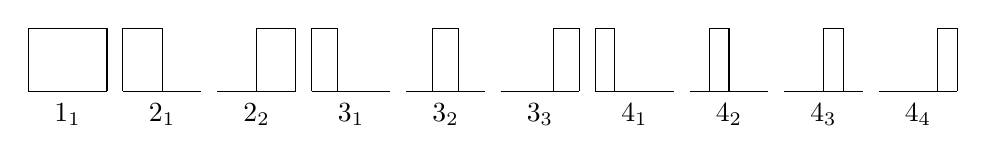
\begin{tikzpicture}
    \draw (-2.3, 0) -- (-1.3, 0); %bottom line
    \draw (-2.3, .8) -- (-1.3, .8); %top line
    \draw (-1.3, .8) -- (-1.3, 0); \draw (-2.3, .8) -- (-2.3, 0); %legs
    \draw (-1.8,-.3) node {$1_1$};

    \draw (-1.1,.8) -- (-.6,.8); \draw (.6, .8) -- (1.1, .8);
    \draw (-1.1, .8) -- (-1.1, 0); \draw(-.6,.8) -- (-.6, 0); \draw (.6, .8) -- (.6, 0); \draw (1.1, .8) -- (1.1, 0);
    \draw (-1.1,0) -- (-.1,0); \draw(.1, 0) -- (1.1,0);
    \draw (-.6,-.3) node {$2_1$};
    \draw (.6,-.3) node {$2_2$};

    \draw (1.3, 0) -- (2.3, 0); %bottom line
    \draw (1.3, .8) -- (1.63, .8); %top line
    \draw (1.3, .8) -- (1.3, 0); \draw (1.63, .8) -- (1.63, 0); %legs
    \draw (1.8,-.3) node {$3_1$};

    \draw (2.5, 0) -- (3.5, 0); %bottom line
    \draw (2.83, .8) -- (3.16, .8); %top line
    \draw (3.16, .8) -- (3.16, 0); \draw (2.83, .8) -- (2.83, 0); %legs
    \draw (3,-.3) node {$3_2$};

    \draw (3.7, 0) -- (4.7, 0); %bottom line
    \draw (4.37, .8) -- (4.7, .8); %top line
    \draw (4.37, .8) -- (4.37, 0); \draw (4.7, .8) -- (4.7, 0); %legs
    \draw (4.2,-.3) node {$3_3$};

    \draw (4.9, 0) -- (5.9, 0); %bottom line
    \draw (4.9, .8) -- (5.15, .8); %top line
    \draw (4.9, .8) -- (4.9, 0); \draw (5.15, .8) -- (5.15, 0); %legs
    \draw (5.4,-.3) node {$4_1$};

    \draw (6.1, 0) -- (7.1, 0); %bottom line
    \draw (6.35, .8) -- (6.6, .8); %top line
    \draw (6.6, .8) -- (6.6, 0); \draw (6.35, .8) -- (6.35, 0); %legs
    \draw (6.6,-.3) node {$4_2$};

    \draw (7.3, 0) -- (8.3, 0); %bottom line
    \draw (7.8, .8) -- (8.05, .8); %top line
    \draw (7.8, .8) -- (7.8, 0); \draw (8.05, .8) -- (8.05, 0); %legs
    \draw (7.8,-.3) node {$4_3$};

    \draw (8.5, 0) -- (9.5, 0); %bottom line
    \draw (9.25, .8) -- (9.5, .8); %top line
    \draw (9.25, .8) -- (9.25, 0); \draw (9.5, .8) -- (9.5, 0); %legs
    \draw (9,-.3) node {$4_4$};
    \end{tikzpicture}
    \end{center}
\end{remark}


\begin{prop}
    A sequence of random variables $\{X_n\}_n$ converges in probability to $X$ if and only if for every subsequence $n(k)$ there exists a further subsequence $\{X_{n(k_j)}\}_j$ that converges almost surely to $X$.
\end{prop}
\begin{proof}
    To prove convergence in probability implies every subsequence has a almost surely convergent further subsequence it is sufficent to check this just for the entire sequence (since any subsequence converges in probability as well).This direction of the proposition is an application of the first Borel-Cantelli Lemma. For all $k \in \mathbb{N}$, there exists an $n_k > n_{k - 1}$ such that,
    \[
        \prob(|X_{n_k} - X| > \frac{1}{k}) < \frac{1}{2^k}
    \]
    Thus since $\sum_{k = 1}^{\infty}\prob(|X_{n_k}- X_n| > \frac{1}{k}) < \infty$, it happens infinitely often with probability 0, therefore converges almost surely.

    To prove the other direction, we first prove the following lemma,
    \begin{lemma}
        Let $y_n$ be a sequence of elements in a topological space. If every subsequence of $y_n$ has a further subsequence that converges to $y$, then $y_n \to y$.
    \end{lemma}
    \begin{proof}
        Suppose $y_n \nrightarrow y$. Then there exists an open neighborhood $y \in U$ that does not contain infinitely many $y_n$. From these we can then construct a subset that does not converge to $y$.
    \end{proof}
    Thus applying this lemma to the sequence $y_n = \prob(|X_n - X| > \vep)$ for all $y$ gives the desired result.
\end{proof}

\begin{cor}
    If $f$ is continuous, $X_n \parrow X$, then $f(X_n) \parrow f(X)$.
\end{cor}

\begin{definition}[Convergence in Distribution/Weak Convergence]
    A sequence of distributions functions $\{F_n\}_n$ converges weakly to a function $F$ (denoted $F \Rightarrow F$) if $F_n(y) \to F(y)$ for all $y$ that are continuity points of $F$. A sequence of random variables $\{X_n\}_n$ converges in distribution to a random variable $X$ (denoted $X_n \Rightarrow X$) if their distribution functions converge weakly to the distribution function of $X$.
\end{definition}
\begin{remark}
    This definition is far weaker than the others. In particular, it is not even required that the random variables all be defined on the same probability space.
\end{remark}


\begin{theorem}
    If $F_n \Rightarrow F$ then there are random variables $Y_n, n \geq 1$ and $Y$ such that $Y_n$ has distribution function $F_n$, $Y$ has distribution function $F$ and $Y_n \xrightarrow{a.s.} Y.$
\end{theorem}
\begin{proof}
    \textcolor{red}{Page 103 in Durrett}
\end{proof}


\begin{theorem}
$X_n \Rightarrow X$ if and only if for every bounded continuous function $g$, we have that $\E[g(X_n)] \to \E[g(X)]$. 
\end{theorem}

\begin{proof}
Let $Y_n$ have the same distribution as $X_n$ and be such that $Y_n$ converges almost surely to $Y \overset{d}{\sim} X$. Since $g$ is continuous we have that $g(Y_n) \to g(Y)$ almost surely and the bounded convergence theorem implies that,
\[\E[g(x_n)] = \E[g(Y_n)] \to \E[g(Y)] = \E(g(X)]\]
To prove the converse, let,
\[g_{x ,\vep}(y) = \begin{cases}
1 & y \leq x\\
0 & y \geq x + \vep\\
\text{linear interpolation} & x \leq y \leq x + \vep
\end{cases}\]
I.e. $g$ is a continuous interpolation between $1_{y \leq x}$ and $1_{y \leq x + \vep}$. Then we have that,
\[\limsup_{n \to \infty} \prob(X_n \leq x) \leq \limsup_{n \to \infty} \E[g_{x,\vep}(X_n)] = \E[g_{x, \vep}(X)] \leq \prob(X \leq x + \vep)\]
Letting $\vep \to 0$, we get $\limsup_{n \to \infty} \prob(X_n \leq x) \leq \prob(X \leq x)$. In the other direction we have that,
\[\liminf_{n \to \infty} \prob(X_n \leq x) \geq \liminf_{n \to \infty} \E[g_{x - \vep, \vep}(X_n)] = \E[g_{x - \vep. \vep}(X)] \geq \prob(X \leq x - \vep)\]
So again we take $\vep \to 0$ and get that $\liminf_{n \to \infty} \prob(X_n \leq x) \geq \prob(X \leq x)$ if $x$ is a continuity point. 
\end{proof}


\begin{theorem}[Helly's Selection Theorem]
    For every sequence $F_n$ of distribution functions, there is a subsequence $F_{n_k}$ and a right continuous nondecreasing function $F$ so that $\lim_{k \to \infty}F_{n_k}(y) = F(y)$ for all continuity points $y$ of $F$. 
\end{theorem}
\begin{proof}
    We begin by making a diagonal argument on the rationals. Letting $q_1, q_2, ...$ be an enumeration of the rationals, we notice that for every $i$, $\{F_n(q_i)\}_n$ is a sequence bounded by $[0,1]$. Therefore we can inductively construct a subsequence $n_{k(i)}$ such that $n_{k(i)}$ is a subsequence of $n_{k(i-1)}$ and $\{F_{n_k(i)}(q_i)\}_{k(i)}$ converges. Then we diagonally construct a subsequence $n_i = n_{i(i)}$ so that for all $q \in \mathbb{Q}$, $\{F_{n_i}(q)\}_i$ converges to some $b_q$. Furthermore, we have that for $p,q \in \mathbb{Q}, p < q$, $b_p < b_q$. We now define,
    \[F(x) = \inf\{b_q| q \in \mathbb{Q}, q > x\}\]
    It is easily verifiable by the monotone property mentioned above that $F(q) = b_q$ and $F$ is right continuous and monotone. Thus all that remains to show is that $F_{n_i}(y) \to F(y)$ for $y$ a continuity point of $F$. By continuity, for every $\vep > 0$ we can select rationals $p, q$ such that $p < y < q$ and,
    \[F(y) - \vep < F(p) \leq F(y) \leq F(q) < F(y) + \vep\]
    Since our subsequence converges on the rationals to $F$, and $F_{n_i}$ is monotone for all $i$, we see that for sufficiently large $i$,
    \[F(y) - \vep < F_{n_i}(p) \leq F_{n_i}(y) \leq F_{n_i}(q) < F(y) + \vep\]
    which concludes the proof.
\end{proof}
\begin{remark}
    Note that this is NOT equivalent to the corresponding measures of the subsequence converging weakly to a measure $\mu$ as $F$ is not necessarily a distribution function (i.e. it may not have the appropriate limits at $\pm \infty$). For a simple example, let $F_n$ be such that $F(x) = 0$ for $x < n$ and $F_n(x) = 1$ for $x \geq n$. Then the resulting pointwise limit $F$ is 0, which is clearly not a probability measure as $
    lim_{x \to + \infty} F(x) \neq 1$. This example illustrates that generally in the limit mass is able to escape to $\pm \infty$ (we could just as easily compute a sequence where mass escapes to $-\infty$ by letting $G_n(x) = F_{-n}(x)$). However, the following definition and theorem gives necessary and sufficient criteria to keep this from happening. 
\end{remark}

\begin{definition}[Tightness]
    A sequence of probaility measures $\mu_n$ on $\R$ is tight if for every $\vep$, there exists a $M_{\vep}$ such that,
    \[\limsup_{n \to \infty} 1 - \mu_n([-M_{\vep}, M_{\vep}]) \leq \vep\]
    Equivalently, a sequence of distribution functions $F_n$ is tight if for every $\vep$ there exists a $M_{\vep}$ such that,
    \[\limsup_{n \to \infty} 1 - F(M_{\vep}) + F(-M_{\vep}) \leq \vep\]
\end{definition}

\begin{theorem}
    A squence of distribution functions $F_n$ is tight if and only if every subsequential limit is the distribution function of a probability measure.
\end{theorem}
\begin{proof}
    Suppose the sequence $F_n$ is tight and $F_{n_k}(y) \to F(y)$ for all continuity points of $F$. Fix some $\vep>0$ and let $r < -M_{\vep}, s > M_{\vep}$. Then we have that,
    \[1 - F(s) + F(r) = \lim_{k \to \infty} 1 - F_{n_k}(s) + F_{n_k}(r) \leq \limsup_{n \to \infty} 1 - F_n(M_{\vep}) + F_n(-M_{\vep}) \leq \vep\]
    This implies that $\limsup_{x \to \infty} 1 - F(x) + F(-x) \leq \vep$. Since $\vep$ was arbitrary and $0 \leq F(-x) \leq F(x) \leq 1$, this implies that $F$ is a probability distribution function.

    To prove the converse, suppose that $F_n$ is not tight. Then there is an $\vep > 0$ and a subsequence such that,
    \[1-F_{n_k}(k) + F_{n_k}(-k) \geq \vep\]
    for all $k$. By choosing a further subsequence, we may assume that there exists a monotone, right continuous $F$ such that $F_{n_k}(y) \to F$ for all continuity points of $F$. Let $r < 0 < s$ be continuity points of $F$. Then we have, 
    \[1 - F(s) + F(r) = \lim_{k \to \infty} 1 - F_{n_k}(s) + F){n_k}(r) \geq \liminf_{k \to \infty} 1 - F_{n_k}(k) + F_{n_k}(-k) \geq \vep\]
    Therefore $F$ cannot be a probability distribution function. 
\end{proof}



\subsection{$L^p$ Space}

\begin{definition}[$L^p$ Space]
$L^p(\om, \cF, \mu)$ is the space of all functions $f: \om \to \R$ such that $||f||_p = (\int |f|^pd\mu)^{1/p}$ is finite. $||f||_{\infty} = \inf\{M \geq 0| \mu(\{x||f(x)|>M\}) > 0\}$ (i.e. $M$ such that $|f|$ is bounded by $M$ almost surely). 
\end{definition}

To illustrate the difference between these norms, note that when $|\om| = 2$, these are all norms on $\R^2$. The following illustrate the circle $\{x \in \R^2| ||x||_p = 1\}$ for various $p$:
\begin{center}
    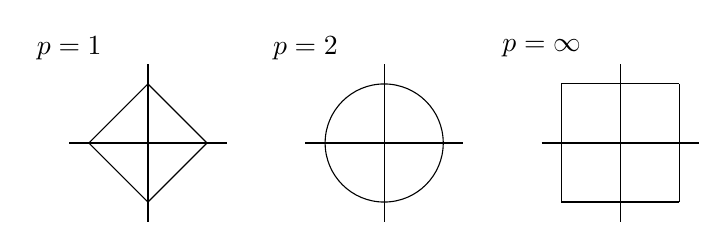
\begin{tikzpicture}
    \draw (-4,0) -- (-2,0); \draw (-3,1) -- (-3,-1); %axes
    % p = 1
    \draw (-3.75, 0) -- (-3, .75); \draw (-3, .75) -- (-2.25, 0); \draw (-2.25,0) -- (-3,-.75); \draw (-3,-.75) -- (-3.75, 0);
    \draw (-4,1.2) node {$p = 1$};
    
    \draw (-1,0) -- (1,0); \draw (0,1) -- (0,-1); %axes
    % p = 2
    \draw (0,0) circle(.75);
    \draw (-1,1.2) node {$p = 2$};
    
    \draw (2,0) -- (4,0); \draw (3,1) -- (3,-1); %axes
    % p = infinity
    \draw (2.25,.75) -- (3.75,.75); \draw (3.75, .75) -- (3.75, -.75); \draw (3.75, -.75) -- (2.25, -.75); \draw (2.25, -.75) -- (2.25, .75);
    \draw (2,1.2) node {$p = \infty$};
    
    \end{tikzpicture}
\end{center}

\begin{theorem}[Minkowski's Theorem]
$||f + g||_p \leq ||f||_p + ||g||_p$.
\end{theorem}
\begin{proof}
\textcolor{red}{Proof needed}
\end{proof}

\begin{theorem}[Riesz-Fischer]
$L^p$ is complete for all $p \in [1, \infty]$
\end{theorem}
\begin{proof}
\textcolor{red}{Proof needed}
\end{proof}

\begin{cor}
$||-||_p$ is a seminorm (fails the 0 only for 0 condition). If we mod out by the relation $f \sim g$ if $f = g$ almost surely, then $||-||_p$ is a Banach space (complete normed vector space).
\end{cor}

The following are some other useful properties of $L^p$ space:
\begin{enumerate}
    \item $L^2$ is a Hilbert Space (a real or complex inner product space that is also a complete metric space).
    \item Embeddings: for $1 \leq p < q \leq \infty$ the following hold:
    \begin{itemize}
        \item $L^q \subset L^p$ if and only if $\om$ does not contain sets of finite but arbitrarily large measure (for instance if $\mu$ is a probability measure).
        \item $L^p \subset L^q$ if and only if $\om$ does not contain sets of nonzero but arbitrarily small measure.
        \item If $\om = \{1,2,...,n\}$, then $L^p \cong L^q \cong \R^n$.
    \end{itemize}
    \item Dual Spaces: For $p,q < \infty$ such that $\frac{1}{p} + \frac{1}{q} = 1$, $L^p$ and $L^q$ are dual to each other as Banach spaces, with identification given by $T_g f = \int fg d\mu$. If $\mu$ is $\sigma$-finite, then $(L^1)^* \cong L^{\infty}$ but we only have that $(L^{\infty})^* \subset L^1$.
    \item For $|\om| = n$, if $p > q$, then $||x||_p \leq ||x||_q \leq n^{1/q - 1/p} ||x||_p$ (and thus they induce the same topology).
\end{enumerate}

\begin{prop}
For $r > s \geq 1$, convergence in $L^r$ implies convergence in $L^s$ but not vice versa.
\end{prop}

\begin{prop}
Both almost sure convergence and $L^p$ convergence imply convergence in distribution
\end{prop}

\subsection{Independence}
\begin{definition}[Independent Sets]
Sets $A_1,..., A_n$ are indpendant if for all $I \subset \{1,...,n\}$, 
\[\prob(\bigcap_{i \in I} A_i) = \prod_{i \in I} \prob(A_i)\]
\end{definition}

\begin{definition}[Independent Random Variables]
Real valued random variables $X_1,...,X_n$ are independent if for all $B_1, ..., B_n \in \cB$,
\[\prob(\bigcap_{i=1}^n\{X_i \in B_i\}) = \prod_{i = 1}^n \prob(X_i \in B_i)\]
An infinite sequence of random variables is said to be independent if every finite subset is independent.
\end{definition}

\begin{definition}[Independent $\sigma$-Algebras]
$\sigma$-algebras $\cF_1,...,\cF_n \subset \cF$ are independent if for all $A_1 \in \cF_i, ..., A_n \in \cF_n$,
\[\prob(\bigcap_{i = 1}^n A_i) = \prod_{i = 1}^n \prob(A_i)\]
\end{definition}

\begin{remark}
Random variables $X_1,..., X_n$ independent is equivalent to the $\sigma$-algebras $\sigma(X_1) ... \sigma(X_n)$ independent.
\end{remark}

\begin{remark}
Pairwise independence is not as strong as collective independence. For instance, let $X_1, X_2, X_3$ be i.i.d $Bernoulli(1/2)$ random variables. Then we have that the following sets are pairwise independent, but not collectively independent:
\[A_1 = \{X_2 = X_3\} \quad A_2 = \{X_1 = X_3\} \quad A_3 = \{X_1 = X_2\}\]
each individually has probability $1/2$, and the intersection of any 2 sets is $\{X_1 = X_2 = X_3\}$ which has probability $1/4$, however the intersection of all 3 is still $\{X_1 = X_2 = X_3\}$ which has probability $1/4 \neq (1/2)^3$.
\end{remark}

\begin{theorem}
For random variables $X_1,...,X_n$, to prove independence it is sufficient to check that for all $x_1,...,x_n \in (- \infty, \infty),$
\[\prob(X_1 < x_1,...,X_n < x_n) = \prod \prob(X_i < x_i)\]
\end{theorem}
\begin{proof}
\textcolor{red}{$\pi-\lambda$ system proof in Durrett}
\end{proof}

\begin{prop}
If $(X_1,...,X_n)$ are absolutely continuous random variables (i.e. they have density $f(x_1,...,x_n)$) then $X_1,...,X_n$ are independent if and only if $f(x_1,...,x_n) = g_1(x_1)...g_n(x_n).$
\end{prop}
\begin{proof}
We can write,
\[\prob(X_1 < x_1, ..., X_n < x_n) = \int_{y_i < x_i} f(y_1,...,y_n)d\Vec{y} = \int_{-\infty}^{x_n} ... \int_{-\infty}^{x_1} g_1(y_1)...g_n(y_n) dy_1...dy_n\]
\[ = \prod_{i = 1}^n (\int_{-\infty}^{x_i} g_i(y_i) dy_i) = \prod_{i = 1}^n \prob(X_i < x_i)\]
\end{proof}

The following are additional properties of independence:
\begin{enumerate}
    \item Functions of independent random variables are independent.
    \item If $X, Y$ are independent with distribution $\mu, \nu$ respectively, and $h: \R^2 \to \R$ is such that either $h \geq 0$ or $\E[|h(X,Y)|] < \infty$, then $\E[h(X,Y)] = \int \int h(x,y) d\mu(x) d\nu(y)$.
    \item If $X_1,...,X_n$ are independent random variables with $X_i \sim \mu_i$, then $(X_1,...,X_n) \sim \mu_1 \times ... \mu_n$
\end{enumerate}

Distribution functions for sums of independent random variables can be given by convolutions of their distribution functions. Let $X$ and $Y$ be independent with $X$ having density function $f$ and $Y$ having density function $g$. Then their sum $X + Y$ has density function,
\[h(z) = (f*g)(z) = \int_{-\infty}^{\infty} f(x) g(z-x) dx = \int_{- \infty}^{\infty} g(y) f(z-y) dy\]
\textcolor{red}{PDFs or CDFs?}

\paragraph{Constructions of Infinite Sequences of Independent Random Variables}
\textcolor{red}{Fill in form page 36 of notes, too tired to do it now}

We now can prove a slightly weaker converse to the first Borel-Cantelli Lemma:

\begin{lemma}[Borel-Cantelli Lemma (2)]
    If $A_n$ are independent, then $\sum_{n = 1}^{\infty} \prob(A_n) = \infty$ implies that $\prob(\limsup_{n \to \infty}A_n) = 1$.
\end{lemma}
\begin{proof}
    We assume the inequality $1 - x \leq e^{-x}$ for $x \in [0,1]$. Then we have that,
    \[\prob((\bigcup_{n = m}^N A_n)^c) = \prob(\bigcap_{n = m}^N A_n^c) = \prod_{n = m}^N (1- \prob(A_n)) \leq e^{-\sum_{n = m}^N \prob(A_n)} \xrightarrow{N \to \infty} 0\]
    Which then implies that $\lim_{N \to \infty} \prob(\bigcup_{n = m}^N A_n) = 1$ for all $m$.
\end{proof}



\subsection{Laws of Large Numbers}
\subsubsection{$L^2$ Law of Large Numbers}
\begin{definition}
    2 random variables $X,Y$ are uncorrelated if $\E[XY] = \E[X]\E[Y]$ or equivalently if,
    \[Cov(X,Y) = \E[(X -\E[X])(Y - \E[Y])] = 0\]
\end{definition}
\begin{remark}
    This is weaker than independence.
\end{remark}

\begin{theorem}[$L^2$ Law of Large Numbers]
    Let $X_1,...,X_n \in L^2(\om)$ be uncorrolated random variables. Then $Var(X_1+ ... + X_n) = Var(X_1)+...+ Var(X_n)$.
\end{theorem}
\begin{proof}
    \textcolor{red}{Proof}
\end{proof}

\begin{remark}
    Note that this implies that if $X_1, X_2,...$ are $i.i.d.$ with variance $Var(X_i) = \sigma^2$, then we have that,
    \[\lim_{n \to \infty} Var(\frac{X_1 + ... + X_n}{n}) = \lim_{n \to \infty} \frac{1}{n^2} Var(X_1 + ... + X_n) = \lim_{n \to \infty} \frac{\sigma^2}{n} = 0\]
    Then we have that $\frac{\sum_{i = 1}^n X_i}{n}$ converges to a constant in $L^2$. Furthermore, convergence in $L^2$ implies convergence in $L^1$, thus $X_n \to \mu$ for $\mu = \E[X_i].$
\end{remark}

\subsubsection{Weak Law of Large Numbers}
\begin{theorem}[Weak Law of Large Numbers]
    Let $X_1, X_2, ...$ be i.i.d. with $\E[|X_i|] < \infty$, and set $S_n = X_1 + ... + X_n$, $\mu = \E[X_i]$. Then as $n \nearrow \infty$, 
    \[\frac{S_n}{n} \xlongrightarrow{p} \mu\]
\end{theorem}
\begin{proof}
    We begin by truncating our random variables $X_i$ by a cutoff $c > 0$. Let $X_i^c = X_i 1_{|X_i| < c}$, and define $Y_i^c = X_i - X_i^c$. Then we have,
    \[\frac{1}{n} \sum_{i = 1}^n X_i = \frac{1}{n} \sum_{i = 1}^n (X_i^c + Y_i^c) = \frac{1}{n} \sum_{i = 1}^n X_i^c + \frac{1}{n} \sum_{i = 1}^n Y_i^c\]
    Let $\xi_n^c = \frac{1}{n} \sum_{i = 1}^n X_i^c$ and $\eta_n^c = \frac{1}{n} \sum_{i = 1}^n Y_i^c$, and define, $a_c = \E[X_i^c], b_c = \E[Y_i^c]$. Then we have,
    \[\delta_n = \E[|\frac{S_n}{n} - \mu|] = \E[|\xi_n^c + \eta_n^c - \mu|] \leq \E[|\xi_n^c - a_c|] + \E[|\eta_n^c - b_c|] \leq \E[|\xi_n^c - a_c|] + 2\E[|Y_i^c|]\]
    Now note that $X_i^c$ is bounded and therefore has finite second moment. Thus, we can apply the $L^2$ law of large numbers and see that $\xi_n^c \xrightarrow{p} a_c$, so we get,
    \[\limsup_{n \to \infty} \delta_n \leq 2\E[|Y_i^c|]\]
    $Y_i^c \xrightarrow{a.s.} 0$, so we can apply dominated convergence theorem with $X_i$ as the bounding variable to see that $2\E[|Y_i^c|] \xrightarrow{c \to \infty} 0$, concluding the proof.

    \textcolor{red}{In my notes I have at the end the phrase "slightly different version with slightly different hypothesis." What is that referring to? Applying the statement of the $L^2$ law of large numbers?}
\end{proof}


\subsubsection{Strong Law of Large Numbers}
We now move onto the strong laws of large numbers, considered strong because they prove almost sure convergence rather than convergence in probability (or $L^2$).
\begin{theorem}[$L^4$ Strong Law of Large Numbers]
    Let $X_i$ be i.i.d. random variables with $\E[X_i] = \mu$ and $\E[X_i^4] < \infty$, then $S_n = X_1 + ... + X_n$, $\frac{S_n}{n} \to \mu$ a.s.
\end{theorem}
\begin{proof}
    We can assume $\mu = 0$ by replacing $X_i$ with $X_i - \mu$. Then we have,
    \[\E[S_n^4] = \sum_{i = 1}^n \E[X_i^4] + \binom{4}{2} \sum_{1 \leq i<j \leq n} \E[X_i^2]\E[X_j^2] = n\E[X_i^4] + 3n(n-1)\E[X_i^2] \leq cn^2\]
    Then we have that 
    \[
        \prob(|S_n| > n \vep) \leq \frac{\E[S_n^4]}{(n\vep)^4} \leq \frac{cn^2}{(n\vep)^4} \leq \frac{1}{n^2 \vep^4}
    \]
    So we have by Borel-Cantelli, $\prob(|S_n| > n \vep \text{ infinitely often}) = 0$
\end{proof}


\begin{theorem}[Strong Law of Large Numbers]
    Let $X_1,X_2,...$ be pairwise independent identically distributed random variables with $\E[|X_i|] < \infty$, $\E[X_i] = \mu$. Then,
     \[ \frac{S_n}{n} \xrightarrow{a.s.} \mu\]
    Additionally, if $\E[X_i^+] = \infty$ and $\E[X_i^-] < \infty$, then $\frac{S_n}{n} \to \infty$ almost surely.
\end{theorem}
We will give two proofs of the strong law of large numbers, the first of which is due to Etemadi in 1981:
\begin{proof}
    \textcolor{red}{need proof of the second statement, should be an application of Borel-Cantelli?}
    Just as in the proof of the weak law of large numbers, we begin by truncating. Let $Y_k = X_k 1_{|X_k|\leq k}$. We first show that it is sufficient to prove the convergence of the truncated variables.
    \begin{lemma}
        Let $T_n = Y_1 + ... + Y_n$. It is sufficient to show that $\frac{T_n}{n} \xrightarrow{a.s.} \mu$.
    \end{lemma}
    \begin{proof}
        $\sum_{k = 1}^{\infty} \prob(|X_k| > k) \leq \int_0^{\infty} \prob(|X_1| > t) dt = \E[|X_i|] < \infty$ so by Borel-Cantelli we have that $\prob(X_k \neq Y_k \text{ infinitely often}) = 0$ Therefore we have that for every $\omega \in \om$ except on a measure $0$ set, there exists a $R(\omega) < \infty$ such that $|S_n(\omega) - T_n(\omega)| < R(\omega)$, so $|\frac{S_n(\omega)}{n} - \frac{T_n(\omega)}{n}| < \frac{R(\omega)}{n} \xrightarrow{n \to \infty} 0.$
    \end{proof}
    \begin{lemma}
        $\sum_{k = 0}^{\infty} \frac{Var(Y_k)}{k^2} \leq 4 \E[X_1] < \infty$
    \end{lemma}
    \begin{proof}
        $Var(Y_k) \leq \E[Y_k^2] = \int_0^{\infty} 2y \prob(|Y_k| > y)dy $\textcolor{red}{why?}$ \leq \int_0^k 2y \prob(|X_1| > y)$ \textcolor{red}{why not equal?}

        Since everything is $\geq 0$, we can apply Fubini's theorem to see,
        \[\sum_{k = 1}^{\infty} \frac{\E[Y_k^2]}{k^2} \leq \sum_{k = 1}^{\infty} 
        \frac{1}{k^2} \int_0^{\infty} 1_{y < k} 2y \prob(|X_1| > k) dy = \int_0^{\infty} (\sum_{k = 1}^{\infty} \frac{1_{y < k}}{k^2}) 2y\prob(|X_1|>y)dy\]
        So to complete the proof we show that if $y \geq 0$, then $2y\sum_{k > y} \frac{1}{k^2} \leq 4$. (For this see Lemma 2.4.4 of Durrett, it is not hard).
    \end{proof}
    Now our goal is to combine these two lemmas to prove the Strong Law of Large Numbers.

    The remainder of this proof follows the following outline:
    \begin{enumerate}
        \item Note that we can write $X_n = X_n^+ - X_n^-$, so we can assume that we are working with $X_i>0$ and combine the results for $X^+$ and $X^-$ to obtain the general case.
        \item Choose a subsequence $T_{k_n}$ and show convergence.
        \item Use the monotonicity to conclude that $T_n$ converges almost surely.
    \end{enumerate}

    To choose the subsequence, For some $\alpha > 1$, define $k_n = [\alpha^n]$ (where $[x]$ is defined to be the closest integer to $x$). Then we have that $k_n$ grows exponentially. So now we have,
    \[\sum_{n = 1}^{\infty} \prob(|T_{k_n} - \E[T_{k_n}]| > \vep k_n) \leq \frac{1}{\vep^2} \sum_{n = 1}^{\infty} \frac{Var(T_{k_n})}{k_n^2} = \frac{1}{\vep^2} \sum_{n=1}^{\infty} \frac{1}{k_n^2} \sum_{m = 1}^{k_n} Var(Y_m) \]
    \[= \frac{1}{\vep^2} \sum_{m = 1}^{\infty} Var(Y_m) \sum_{k_n \geq m} \frac{1}{k_n^2} \leq 4(1-\frac{1}{\alpha^2})^{-1}\frac{1}{\vep^2}\sum_{m = 1}^{\infty} \frac{\E[Y_m^2]}{m^2} < \infty\]
    Thus by Borel-Cantelli we can conlude that,
    \[ \frac{T_{n_k} - \E[T_{n_k}]}{n_k} \xrightarrow{a.s.} 0\]
    Note that this is sufficient to show this subsequence converges to $\mu$ as this implies that,
    \[\lim_{k \to \infty} \frac{T_{n_k}}{n_k} = \lim_{k \to \infty} \frac{\E[T_{n_k}]}{n_k} = \lim_{k \to \infty} \frac{\E[S_{n_k}]}{n_k}  = \mu\]

    Now to handle the intermediate values we have the following inequality for $k_n \leq m \leq k_{n+1}$:
    \[\frac{T_{k_n}}{k_{n+1}} \leq \frac{T_m}{m} \leq \frac{T_{k_{n+1}}}{k_n}\]
    So then this implies that,
    \[(\frac{k_{n}}{k_{n+1}})\frac{T_{n_k}}{n_k} \leq \frac{T_m}{m} \leq (\frac{k_{n+1}}{k_n})\frac{T_{k_{n+1}}}{n_{k+1}}\]
    and by our choice of subsequence we have that $\frac{k_{n+1}}{k_n} \to \alpha$ as $n \to \infty$, for arbitrarily chosen $\alpha > 1$, thus,
    \[\mu \leq \liminf_{m \to \infty} \frac{T_m}{m} \leq \limsup_{m \to \infty} \frac{T_m}{m} \leq \mu\]
    which concludes the first proof.
\end{proof}

To present the second proof we first need to prove the following theorems of Kolmogorov:

\begin{theorem}[Kolmogorov's Maximal Inequality]
    Let $X_1, X_2,...$ be independent centered random variables with $Var(X_i) < \infty$. Let $S_n = X_1 + ... + X_n$. Then,
    \[
        \prob(\max_{1 \leq k \leq n} |S_k| \geq x) \leq \frac{Var(S_n)}{x^2}
    \] 
\end{theorem}
\begin{remark}
    Note that this is stronger than the Chebyshev inequality since we take the maximum over all $S_k$ for $k \leq n$.
\end{remark}
\begin{proof}
    Define $A_k = \{|S_k| \geq x, |S_j| < x \text{ for all } j < k\}$. Note that the $A_k$ are disjoint, and that $\bigcup_{k = 1}^n A_k = \{\max_{1 \leq k \leq n} |S_k| \geq x\}$. Then we have,
    \[\E[S+n^2] = \sum_{k =1}^n \int_{A_k} S_n^2 d \prob ... \]
    \textcolor{red}{UNFINISHED IN MY NOTES see Durrett to finish}
\end{proof}

\begin{theorem}[Kolmogorov 0-1 Law]
    Define $\cF_n' = \sigma(X_n, X_{n+1},...)$ the smallest $\sigma$-field such that all $X_m, m \geq n$ are measurable. Define the tail $\sigma$-field $\mathcal{T}= \bigcap_{n = 1}^{\infty}$. If the sequence $X_1, X_2, ...$ are independent, then for an $A \in \mathcal{T}$, $\prob(A) = 0$ or $1$.
\end{theorem}

\begin{proof}
    The idea of the proof is to show that $A$ is independent from itself and therefore must have probability either 0 or 1. This requires $\pi = \lambda$ systems and can be found in Durrett \textcolor{red}{REVISIT IF YOU EVER GET AROUND TO $\pi-\lambda$ STUFF}
\end{proof}

We use these two theorems to prove the following theorem that we will the apply to give a second proof of the Strong Law of Large Numbers.

\begin{theorem}[Kolmogorov's One Series Theorem]
    Suppose $X_1, X_2,...$ are independent centered random variables. If $\sum_{i = 0}^{\infty} Var(X_i) < \infty$, then with probability 1,
    \[\sum_{i = 1}^{\infty} X_i(\omega)\]
    converges.
\end{theorem}
\begin{proof}
    Let $S_n$ be the $n$-th partial sum of the series. To prove this we will prove
    $$\prob(\{S_n\}_n \text{ is Cauchy})= 1$$
    By Kolmogorov's maximal inequality we have,
    \[\prob(\max_{M \leq m \leq N}|S_m - S_M| > \vep) \leq \frac{1}{\vep^2} Var(S_N- S_M) = \frac{1}{\vep^2} \sum_{n = M+1}^N Var(X_n) < \infty\]
    So we have,
    \[\prob(\sup_{m,n \geq M} |S_m - S_n| > 2\vep) \leq \prob(\sup_{m \geq M} |S_m - S_M| > \vep) \xrightarrow{M \to \infty} 0\]
\end{proof}

We also will need the following lemma, which we won't prove here,

\begin{lemma}[Kronecker's Lemma]
    If $a_n \to \infty$ and $\{x_n\}_n$ is such that $\sum_{i = 1}^{\infty} \frac{x_n}{a_n}$ converges then $\frac{1}{a_n} \sum_{i = 1}^n x_n \xrightarrow{n \to \infty} 0$.
\end{lemma}

Now we give the second proof of the Strong Law of Large Numbers:
\begin{proof}
    Again, let $Y_k = X_k1_{|X_k| \leq k}$, and let $Z_k = Y_k - \E[Y_k]$. Recall that by lemma 4 of proof 1 it is sufficient to show to show that $\frac{T_n - \E[T_n]}{n} \to 0$ almost surely. We have, $Var(\frac{Z_k}{k}) = \frac{Var(Y_k)}{k^2} < \infty$ by lemma 5 in the first proof, therefore by Kolmogorov's one series theorem, $\sum_{k = 1}^{\infty} \frac{Z_k}{k}$ converges almost surely. By Kronecker's lemma, this implies that $\frac{1}{n} \sum_{k = 1}^n Z_k \to 0$ almost surely, so, 
    \[\frac{1}{n} \sum_{k = 1}^n Z_k = \frac{\sum_{k = 1}^nY_k - \E[Y_k]}{n}= \frac{T_n - \E[T_n]}{n} \xrightarrow{a.s.} 0\]
\end{proof}

\subsubsection{Applications}
The following are examples of applications of the laws of large numbers chosen from Durrett,

\paragraph{Bernstein Polynomials}
Let $f$ be continuous on $[0,1]$, and define the \textit{$n$-th Bernstein polynomial of $f$} to be,
\[ f_n(x) = \sum_{m = 0}^n \binom{n}{m} x^m(1-x)^{n-m} f(\frac{m}{n}) \]
Then $\sup_{x \in I}|f_n(x) - f(x)| \xrightarrow{n \to \infty} 0$.

\begin{proof}
    Let $X_i \sim Bern(p)$, $S_n = X_1 + ... + X_n$, then we have that, $\prob(S_n = m) = \binom{n}{m} p^m(1-p)^{n-m}$. Therefore,
    \[f_n(p) = \E[f(\frac{S_n}{n})] \xrightarrow{n \to \infty} f(p)\]
\end{proof}


\paragraph{High-Dimensional Cubes Concentrate on the Boundary of a Ball} 
Let $X_i \sim Unif[-1,1]$, $Y_i = X_i^2$, Then we can easilyt see that $\E[Y_i] = \frac{1}{3}$ and $Var(Y_i) \leq 1$. Thus by the law of large numbers we have,
\[\frac{X_1^2+...+X_n^2}{n} \xrightarrow{n \to \infty} \frac{1}{3}\]
Therefore, by the law of large numbers, for some small $\delta > 0$, the $\delta$-neighborhood of the ball $B(0, \sqrt{\frac{n}{3}})$ contains almost all of the mass of the cube.

\begin{comment}
\paragraph{Record Values}
Let $X_1, X_2, ... $ be i.i.d. random variables distributed according to some continuous distribution. Let $A_k$ be the event that $X_k$ sets a record, that is, $A_k = \{X_k > \sup_{j \leq k} X_j\}$. Perhaps unintuitively, the $A_k$ are independent events, and $\prob(A_k) = \frac{1}{k}$

\begin{proof}
    For every $n$ we can define the random variable $\pi \in S_n$ such that $\pi(\omega)$ is such that $X_{\pi(\omega)(1)} \leq ... \leq X_{\pi(\omega)(n)}$. By the $i.i.d.$ property of the $X_i$'s, $\pi$ is uniform on $S_n$, so $\prob(A_n) = \prob(\pi(n) = n) = \frac{1}{n}$
\end{proof}
\end{comment}

\paragraph{Renewal Theorem} Let $X_1, X_2, ... $ be i.i.d. random bariables with $0 < X_i < \infty$. Define $T_n = X_1 + ... + X_n$ and let $\E[X_i] = \mu$. Define $N_t = \sup\{n| T_n \leq t\}$ By the law of large numbers we have that $\frac{S_n}{n} \xrightarrow{a.s.} \mu$, and we claim that $\frac{N_t}{t} \xrightarrow{a.s.} \frac{1}{\mu}$.
\begin{proof}
    $T_{N_t} \leq t \leq T_{N_t + 1}$, so
    \[\frac{T_{N_t}}{N_t} \leq \frac{t}{N_t} \leq \frac{T_{N_t + 1}}{N_t+1} (\frac{N_t + 1}{N_t})\]
    Both the right hand side and left hand side go to $\mu$ as $t \to \infty$ by the law of large numbers so we are done.
\end{proof}


\paragraph{Triangular Arrays}
\textcolor{red}{Page 51 in Durrett}


\subsection{Central Limit Theorem}
\subsubsection{Characteristic Functions}
\begin{definition}[Characteristic Function]
    For a random variable $X$ with distribution $\mu$ on $\R$ and $t \in \R$, the characteristic function $\varphi_X(t)$ is defined to be,
    \[\varphi_X(t) = \E[e^{itX}] = \int_{\R} e^{itX} d\mu\]
\end{definition}

The following are easily verifyable properties of characteristic functions:

\begin{enumerate}
    \item $\vp_X(0) = 1$
    \item $\vp_X(-t) = \overline{\vp_X(t)}$
    \item $|\vp_X(t)| = |\E[e^{itX}]| \leq \E[|e^{itX}|] = \E[1] = 1$
    \item $\vp_X$ is uniformly continuous on $(-\infty, \infty)$: $$|\vp_X(t) - \vp_X(t + h)| = |\E[e^{itX}(1-e^{ihX})]| \leq \E[|1-e^{ihX}|]$$
    \item $\vp_{aX+b}(t) = \E[e^{it(aX+b)}] = e^{itb}\vp_X(at)$
    \item If $X \in \mathbb{Z}$ almost surely, $\vp_X(t + 2\pi) \vp_X(t):$ $$\vp_X(t+2\pi) = \E[e^{i(t+2\pi)X}] = \E[e^{i2\pi X}e^{itX}] = \vp_X(t)$$
\end{enumerate}

\begin{prop}
    If $X_1$ and $X_2$ are independent, then $\vp_{X_1+X_2}(t) = \vp_{X_1}(t)\vp_{X_2}(t)$
\end{prop}
\begin{proof}
    We can check this directly,
    \[\vp_{X_1 +X_2}(t) = \E[e^{it(X_1+X_2)}] = \E[e^{itX_1}e^{itX_2}] = \E[e^{itX_1}] \E[e^{itX_2}] = \vp_{X_1}(t) \vp_{X_2}(t) \]
\end{proof}

\begin{example}[Bernoulli($\frac{1}{2}$)]
    If $X \sim Bern(\frac{1}{2})$, then, $$\vp_{X}(t) = \frac{1}{2}e^{it} + \frac{1}{2}e^{-it} = \cos(t)$$
    For general $p$, $\vp_X(t) = pe^{it} + (1-p)e^{-it}$.
\end{example}

\begin{example}[Binomial($n, \frac{1}{2}$)]
    By proposition 13 and example 3, we have that for $X \sim Bin(n, \frac{1}{2})$, 
    \[\vp_X(t) = \cos^n(t)\]
\end{example}

\begin{example}[Poisson($\lambda$)]
    If $N \sim Po(\lambda)$, then,
    \[\vp_N(t) = \sum_{k = 0}^{\infty} e^{itk}e^{-\lambda} \frac{\lambda^k}{k!} = e^{-\lambda} \sum_{k = 0}^{\infty}\frac{(e^{it} \lambda)^k}{k!} = e^{\lambda(e^{it}-1)}\]
\end{example}

\begin{example}[Normal($0, \sigma^2$)]
    For $Z \sim \cN(0, \sigma^2)$,
    \[\vp_Z(t) = \frac{1}{\sigma \sqrt{2\pi}}\int_{-\infty}^{\infty} e^{itx}e^{-x^2/2\sigma^2} dx = e^{-\sigma^2t/2} \]
\end{example}

\begin{example}[Uniform]
    For $U \sim Unif[a,b]$,
    \[\vp_U(t) \frac{1}{it(b-a)}(e^{itb} - e^{ita})\]
    If $a = c$ and $b = -c$, then we have that,
    \[\vp_U(t) = \frac{\sin(ct)}{ct}\]
\end{example}

\begin{example}[Triangle Density]
    For $X$ a random variable with density $f(x) = 1-|x|$ on $[-1,1]$ (example: $U_1 + U_2$ for $U_1,U_2$ independent $\sim Unif[-1/2,1/2]$),
    \[\vp_X(t) = \vp_{U_1}(t)vp_{U_2}(t) = (\frac{\sin^2(t/2)}{t/2})^2 = \frac{2(1-\cos(t))}{t^2}\]
\end{example}

\begin{example}[Exponential]
    For $X \sim exp(\lambda)$,
    \[\vp_X(t) = \lambda \int_0^{\infty} e^{itx}e^{-\lambda x}dx = \frac{\lambda}{(it- \lambda)}\]
\end{example}

Now the question becomes, how do we reverse this process? That is, how can we recover a distribution from a characteristic function?

\begin{theorem}[Inversion Formula for Characteristic Functions]
    Let $\vp(t) = \int_{\R} e^{itx}\mu(dx)$ for $\mu$ a probability distribution. Then for $a < b$, 
    \[\mu((a,b)) + \frac{1}{2}\mu(\{a,b\}) = \lim_{T \to \infty} \frac{1}{2\pi} \int_{-T}^T \frac{e^{-ita} - e^{-itb}}{it}\vp(t)dt\]
\end{theorem}
\begin{proof}
    Define,
    \[I_t = \int_{-T}^T \frac{e^{-ita} - e^{-itb}}{it}\vp(t)dt = \int_{-T}^{T} \int_{\R} \frac{e^{-ita} - e^{-itb}}{it}e^{itx} \mu(dx) dt\]
    To show that this integral exists, we observe that,
    \[\frac{e^{-ita} - e^{-itb}}{it} = \int_a^b e^{-ity}dy\]
    Therefore, $|\frac{e^{-ita} - e^{-itb}}{it}| \leq b - a$.

    Since $\mu$ is a probability measure and $[-T,T]$ is a finite interval we are allowed to apply Fubini's theorem to obtain,
    \[I_T = \int_{\R} \int_{-T}^T \frac{e^{-ita} - e^{-itb}}{it} e^{itx} dt \mu(dx)\]
    \[= \int_{\R}(\int_{-T}^T \frac{\sin(t(x-a))}{t}dt - \int_{-T}^T\frac{\sin(t(x-b))}{t}dt)\]
    Define,
    \[R(\theta,T) = \int_{-T}^T \frac{\sin(t\theta)}{t} dt \quad \quad \quad S(T) = \int_0^T \frac{\sin(x)}{x} dx\]
    Then we have that
    \[I_T = \int_{\R}(R(x - a, T) - R(x-b, T))\mu(dx)\]
    Apply a change of variables letting $t = x/\theta$ to get,
    \[R(\theta,T) = 2\int_0^{T\theta} \frac{\sin(x)}{x} dx = 2S(T\theta)\]
    Since $\sin$ is an odd function, we have that $R(\theta,T) = sgn(\theta)R(|\theta|,T)$, so we get that $R(\theta,T) = 2sgn(\theta)S(T|\theta|)$
    As $T \to \infty$, $S(T) \to \pi/2$ (See exercise 1.7.5 in Durrett). This implies that $\lim_{T \to \infty} R(\theta,T) = \pi sgn(\theta)$, therefore we get that,
    \[\lim_{T \to \infty} R(x - a,T) - R(x-b,T) = \begin{cases}
        2\pi & a < x < b\\
        \pi & x = a \text{ or } x = b\\
        0 & \text{else}
    \end{cases}\]
    We then use dominated  convergence to bring the limit inside of the integral to get,
    \[\lim_{T \to \infty} \frac{1}{2\pi} \int_{\R} (R(x - a, T) - R(x - b, T))\mu(dx) = \frac{1}{2\pi}(\int_a^b 2\pi \mu(dx) + \pi(\mu(a) + \mu(b))\]
    \[= \mu((a,b)) + \frac{1}{2}\mu(\{a,b\})\]
\end{proof}

The following theorem about inverting point masses won't be proven here but follows a similar structure to the inversion theorem proof above:

\begin{theorem}
    If $\vp(t) = \int_{\R} e^{itx}\mu(dx)$, then 
    \[\mu(\{a\}) = \lim_{T \to \infty} \frac{1}{2T} \int_{-T}^T e^{-ita} \varphi(t)dt\]
\end{theorem}

\begin{cor}
    If $\vp_X$ is real, then $X$ and $-X$ have the same  distribution.
\end{cor}

\begin{cor}
    If $X_1 \sim \cN(0, \sigma^2_1), X_2 \sim \cN(0, \sigma^2_2)$ are independent, then $X_1 + X_2 \sim \cN(0, \sigma_1^2 + \sigma_2^2)$
\end{cor}

\begin{theorem}
    If $\int|\varphi(t)|dt < \infty$, then $\mu$ has bounded continuous density,
    \[f(y) = \frac{1}{2\pi} \int e^{ity} \vp(t)dt\]
\end{theorem}
\begin{proof}
    By the bound on the integrand mentioned in the inversion theorem and the fact that our integral converges absolutely, we have that,
    \[\mu((a,b)) + \frac{1}{2}\mu(\{a,b\}) = \int_{-\infty}^{\infty} \frac{e^{-ita} - e^{-itb}}{it} \vp(t)dt \leq \frac{(b-a)}{2\pi} \int_{-\infty}^{\infty} |\vp(t)|dt \xrightarrow{a \to b} 0\]
    which implies that $\mu$ has no point masses. 

    Next, we have that,
    \[\mu((x,x+h)) = \frac{1}{2\pi} \int \frac{e^{-itx} - e^{-it(x+h)}}{it}\vp(t)dt = \frac{1}{2\pi} \int (\int_x^{x + h} e^{-ity} dy) \vp(t) dt\]
    \[ = \int_x^{x + h} (\frac{1}{2\pi} \int e^{-ity}\vp(t)dt) dy\]
    Therefore $\mu$ has density function,
    \[f(y) = \frac{1}{2\pi} \int e^{-ity}\vp(t)dt\]
\end{proof}

\begin{prop}
    Let $X$ be a random variable with distribution $\mu$. If $\int|x|^n \mu(dx) < \infty$, then,
    \begin{enumerate}
        \item  $\vp_X^{(n)}(0) = i^n \E[X^n]$
        \item $\vp_X(t) = \sum_{m = 0}^n \frac{1}{m!} \E[(itX)^m] + g_n(t)$ for $g_n(t) = o(t^n)$.
        \item $|g_n(t)| \leq \E[\min(|tX|^{n+1}, 2|tX|^n)]$
    \end{enumerate}
\end{prop}
\begin{proof}
    1 follows from the fact that $\vp_X^{(n)}(t) = \int (ix)^n e^{itx} \mu(dx)$. 2 follows from taylor expanding $\vp_X$. 

    \textcolor{red}{why is 3 true?}
\end{proof}

\begin{theorem}[Levy-Cramer Continuity Theorem]
    Let $\mu_n, n \geq 1$ be probability measures with characteristic functions $\vp_n$. Then (i) if $\mu_n \Rightarrow \mu$, $\vp(t) \to \vp(t)$ for $\vp$ the characteristic function of $\mu$. (ii) If $\vp_n(t)$ converges pointwise to a limit $\vp(t)$ that is continuous at $0$, then the associated sequence of probability measures is tight and converges weakly to the measure $\mu$ with characteristic function $\vp$.
\end{theorem}
\begin{proof}
    We will first prove (i). Recall from theorem 10 that $\mu_n \Rightarrow \mu$ if and only if for every bounded continuous function $g$, $
    int g(x)\mu_n(dx) \to \int g(x) \mu(dx)$. We have that,
    \[\vp_n(t) = \int e^{itx} \mu_n(dx) = \int \cos(tx) \mu_n(dx) + i \int \sin (tx) \mu_n(dx)\] \[\xrightarrow{n \to \infty} \int \cos(tx) \mu(dx) + i\int \sin(tx)\mu(dx) = \vp(t)\]
    Where the limit follows by applying theorem 10 with $g(x) = \cos(tx)$ and $g(x) = \sin(tx)$.

    Next we prove (ii). First, we claim that the convergence of characteristic functions implies that $\mu_n$ is tight (see page 115 of Durrett for details on the proof).

    Next, we apply Helly's selection theorem and theorem 12 to obtain a subsequence $\mu_{n_k}$ such that $\mu_{n_k} \Rightarrow \mu$ for $\mu$ a probability measure on $\R$. It is clear from (i) that this then implies $\mu$ has distribution function $\vp$. This observation and tightness then implies that every sequence has a further subsequence that converges to $\mu$. We now use theorem 10 to prove that this implies $\mu_n \Rightarrow \mu$. Suppose $f$ is continuous and bounded. Then we know that every subsequence of $\{\int f(x) \mu_n(dx)\}_n$ has a further subsequence that converges to $\int f(x) \mu(dx)$, therefore $\int f(x) \mu_n(dx) \to \int f(x) \mu(dx)$, which concludes the proof.
\end{proof}

\textcolor{red}{Higher dimensional characteristic functions and inversion formula/sufficient conditions to check weak convergence}

\subsubsection{The Central Limit Theorem and Variations}

\begin{theorem}[The Central Limit Theorem]
    Let $X_1, X_2, ...$ be i.i.d. random variables with $\E[X_i] = \mu$ and $Var(X_i) = \sigma^2$. Let $Z \sim \cN(0,1)$, then
    \[\frac{S_n - n\mu}{\sigma \sqrt{n}} \Rightarrow Z\]
\end{theorem}
\begin{proof}
    By centering, we can assume that $\mu = 0$. We will prove this theorem by proving that the characteristic functions $\vp_{\frac{S_n}{\sigma \sqrt{n}}}(t)$ converge pointwise to the characteristic function of $Z$, $\vp_{Z}(t) = e^{-t/2}$.
    \begin{align*}
        \vp_{\frac{S_n}{\sigma \sqrt{n}}}(t) & = \E[e^{it\frac{S_n}{\sigma \sqrt{n}}}]\\
        & = (\E[e^{it\frac{X_i}{\sigma \sqrt{n}}}])^n & \text{By } \{X_k\}_k \text{ i.i.d}\\
        & = (1 - \frac{1}{2}(\frac{t}{\sigma\sqrt{n}})^2 \sigma^2 + o(\frac{t^2}{\sigma^2n}))^n & \text{By Proposition 14}\\
        & = (1 - \frac{t}{2n} + o(\frac{1}{n}))^n
    \end{align*}
    We then apply the following lemma to the above formula (which we won't prove here):
    \begin{lemma}
        If $c_j \to 0$, $a_j \to \infty$, and $c_ja_j \to \lambda$, then $(1+c_j)^{a_j} \to e^{\lambda}$
    \end{lemma}
    Taking $a_j = j$, and $c_j = -\frac{t}{2j} + o(\frac{1}{j})$, we have that $\lambda = -\frac{t}{2}$, so,
    \[\lim_{n \to \infty} \vp_{\frac{S_n}{\sigma \sqrt{n}}}(t) = \lim_{n \to \infty} (1 - \frac{t}{2n} + o(\frac{1}{n}))^n = e^{-\frac{t}{2}} = \vp_Z(t)\]
\end{proof}

\textcolor{red}{COME BACK TO THIS SECTION AND SAY MORE (pg 58 in notes)}

\textcolor{red}{Weak convergence in general metric spaces and the Protmanteau theorem}

\begin{theorem}[Cramér-Wold Device]
    Let $\{X_n\}_n$ be a sequence of random vectors in $\R^d$ such that for all $\theta \in \R^d$, $X_n \cdot \theta \Rightarrow X \cdot \theta$, then $X_n \Rightarrow X$
\end{theorem}
\begin{proof}
    Let $\vp_n$ and $\vp$ be the characteristic functions of $X_n$ and $X$ respectively. Then for all $\theta \in \R^d$ we have,
    \[\vp_n(\theta) = \vp_{\theta \cdot X_n}(1) \xrightarrow{n \to \infty} \vp_{\theta \cdot X}(1) = \vp(\theta)\]
\end{proof}

\begin{theorem}[Central Limit Theorem in $\R^d$]
    Let $X_1,X_2,...$ be i.i.d. random vectors in $\R^d$ with $\E[X_i] = \mu \in \R^d$ and covariance matrix $\Gamma_{i,j} = \E[(X_k^i - \mu_i)(X_k^j - \mu_j)]$. Let $X$ be a multivariate Gaussian random vector in $\R^d$ with $\E[X] = 0$ and covariance matrix $\Gamma$, and define $S_n = X_1 + ... + X_n$. Then,
    \[\frac{S_n-\mu n}{\sqrt{n}} \Rightarrow X\]
\end{theorem}

We now will state a theorem that gives bounds on the rate of convergence of these sequences of random variables to the normal distribution.

\begin{theorem}
    Let $X_1, X_2, ...$ be i.i.d. random variables in $\R$ with $\E[X_i] = 0, \E[X_i^2] = \sigma^2$, and let $F_n$ be the distribution function for $\frac{S_n}{\sigma \sqrt{n}}$. Denote $\Phi(x) = \frac{1}{\sqrt{2\pi}} \int_{-\infty}^x e^{-y^2/2} dy$ the distribution function of $\cN(0,1)$, then,
    \[\sup_x|F_n(x) - \Phi(x)| \leq \frac{3 \E[|X_i|^3]}{\sigma^3\sqrt{n}}\]
\end{theorem}
\textcolor{red}{Maybe prove this but probably not}

\textcolor{red}{Local Limit CLT}

The following theorem gives us nice control on the magnitude of fluctuations of a random walk.

\begin{theorem}[Law of the Iterated Logarithm]
    Let $X_1, X_2, ...$ be i.i.d. random variables with $\E[X_i] = 0$ and $\E[X_i^2] = 1$. Then,
    \[\limsup_{n \to \infty}|\frac{S_n}{\sqrt{n\log(n)}}| = \sqrt{2} \text{  a.s.}\]
\end{theorem}
\begin{proof}
    \textcolor{red}{Proof}
\end{proof}

\subsection{Markov Chains}
\subsubsection{Condition Expectation}
\begin{definition}[Conditional Expectation]
    Let $X$ be a random variable on $(\om, \cF, \prob)$ with $\E[|X|]< \infty$, $\Sigma$ a $\sigma$-subalgebra of $\cF$. Then $\E[X|\Sigma]$ is any $\Sigma$-measurable random variable satisfying,
    \[\int_{A} \E[X|\Sigma] d\prob = \int_A X d\prob\]
    for all $A \in \Sigma$.
\end{definition}
\begin{remark}
    The existence and uniqueness up to a measure 0 set of this construction will be assumed for now and proven later. \textcolor{red}{MAKE SURE THIS IS PROVEN LATER IN RN SECTION}
\end{remark}

\begin{prop}
    Conditional expectation satisfies the following properties,
    \begin{enumerate}
        \item If $X$ is $\Sigma$-measurable, then $\E[X|\Sigma] = X$.
        \item $\E[\E[X|\Sigma]] = \E[X]$
        \item If $X \geq 0$, then $\E[X|\Sigma] \geq 0$ almost surely.
        \item $\E[a_1X_1 + a_2X_2|\Sigma]= a_i \E[X_i|\Sigma] + a_2\E[X_2|\Sigma]$
        \item If $Z$ is $\Sigma$-measurable and bounded then $\E[ZX|\Sigma] = Z\E[X|\Sigma]$ almost surely.
        \item If $Z$ is a bounded $\Sigma$-measurable random variable, then $\E[Z\E[X|\Sigma]] = \E[ZX]$.
        \item If $\Sigma' \subset \Sigma \subset \cF$, then $\E[\E[X|\Sigma]|\Sigma'] = \E[X|\Sigma']$
        \item Conditional Jensen's Inequality: If $\vp$ is a convex real valued function, then $\vp(\E[X|\Sigma]) \leq \E[\vp(X)|\Sigma]$
    \end{enumerate}
\end{prop}
\begin{proof}
    1 follows trivially from the definiton. For 2, we take $A = \om$ and see that from the definition,
    \[\E[\E[X|\Sigma]] = \int_{\om}\E[X|\Sigma] d \prob = \int_{\om} X d \prob = \E[X]\]

    For 3, we let $A = \E[X|\Sigma]^{-1}(-\infty, 0)$. Notice that since $(-\infty, 0) \in \cB$, $A \in \Sigma$. Therefore we know that,
    \[0 \geq \int_A \E[X|\Sigma]d\prob = \int_A X d \prob \geq 0\]
    Thereofore $\int_A\E[X|\Sigma]d\prob = 0$ and since $\E[X|\Sigma] < 0$ on $A$, this implies that $\prob(A) = 0$.

    To prove 4, first notice that the left hand side is clearly $\Sigma$-measurable, so it satisfies the first condition of the definition. To check the second condition, we let $A \in \Sigma$ and observe,
    \[\int_A a_1X_1 + a_2X_2 d\prob = a_1\int_A X_1 d \prob + a_2\int X_2d\prob\] \[ = a_1 \int \E[X_1|\Sigma] d \prob + a_2 \int \E[X_2|\Sigma] d\prob = \int a_1 \E[X_1|\Sigma] + a_2 \E[X_2|\Sigma] d \prob\]

    To prove 5, we use simple functions to approximate $Z$ from below via the following formula. Let $M$ be such that $|Z| \leq M$,
    \[\vp_n = \sum_{k = -nM}^{nM-1} \frac{k}{n} 1_{Z^{-1}([\frac{k}{n}, \frac{k+1}{n}))}\]
    Therefore we have that $\vp_n(\omega) \leq Z(\omega) < \vp(\omega) + \frac{1}{n}$ and furthermore, note that because $Z$ is $\Sigma$-measurable, $Z^{-1}([\frac{k}{n},\frac{k+1}{n})) \in \Sigma$. We know that $|\vp_n X| \leq M|X|$, so for any $A \in \Sigma$, we can apply the dominated convergence theorem to see that,
    \[\int_A Y \E[X|\Sigma] d\prob = \lim_{n \to \infty} \int \vp_n \E[X|\Sigma] d \prob = \lim_{n \to \infty} \sum_{k = -nM}^{nM - 1} \frac{k}{n} \int_{A \cap Z^{-1}[\frac{k}{n}, \frac{k_1}{n})]}\E[X|\Sigma]d\prob\]
    \[= \lim_{n \to \infty} \sum_{k = -nM}^{nM - 1} \frac{k}{n} \int_{A \cap Z^{-1}[\frac{k}{n}, \frac{k_1}{n})]}Xd\prob = \lim_{n \to \infty} \int \vp_n X d\prob = \int YX d \prob\]
    So $Y \E[X|\Sigma]$ is $\Sigma$ measurable and satisfies $\int_A Y\E[X|\Sigma]d\prob = \int_A YX d\prob$ for all $A \in \Sigma$. 6 then follows from 5 and 2. 

    For 7, we observe that for $A \in \Sigma' \subset \Sigma$,
    \[\int_A \E[\E[X|\Sigma]|\Sigma'] d\prob = \int_A \E[X|\Sigma]d\prob = \int_A X d\prob\]

    Lastly, to prove the conditional Jensen's inequality, notice that for $\vp$ convex, we can write,
    \[\vp(x) = \max_{\substack{h \leq \vp\\h \text{ linear}}} h(x)\]
    By property 4 for any $h \leq \vp$ we have
    \[\E[\vp(X)|\Sigma] \geq \E[h(X)|\Sigma] = h(\E[X|\Sigma])\]
    which implies,
    \[\E[\vp(X)|\Sigma] \geq \max_{\substack{h \leq \vp \\ h \text{ linear}}} h(\E[X|\Sigma]) = \vp(\E[X|\Sigma])\]
\end{proof}

The following examples should help to connect this definition of conditional expectation with our usual understanding. Intuitively, we want to think of $\Sigma$ as information we know.

\begin{example}[No Information]
    Suppose that $X$ is such that $\sigma(X)$ is independent from $\Sigma$. Then in this case, $\E[X|\Sigma] = \E[X]$. To see this, note that for any $A \in \Sigma$, $X$ and $1_A$ are independent, therefore,
    \[\int_A X d \prob = \E[X1_A] = \E[X]\E[1_A] = \int_A \E[X]d \prob\]
\end{example}

\begin{example}[Averaging]
    Let $\om_1, \om_2, ...$ be a (finite or infinite) partition of $\om$ into disjoint sets of positive measure, and let $\Sigma = \sigma(\om_1, \om_2, ...)$. Then for $\omega \in \om_i$, we have,
    \[\E[X|\Sigma] = \frac{\E[X1_{\om_i}]}{\prob(\om_i)} = \frac{\int_{\om_i} Xd\prob}{\prob(\om_i)}\]
    So in words, in this case $\E[X|\Sigma]$ is the random variable such that it's value on $\omega \in \om_i$ is the average of $X$ over $\om_i$. 
\end{example}

\begin{example}[Conditioning on a Random Variable]
    For random variables $X$ and $Y$ we can obtain the usual definiton of $\E[X|Y]$ from our definition by taking $\E[X|Y] = \E[X|\sigma (Y)]$.
\end{example}

\begin{prop}
    Suppose that $X$ and $Y$ are random variables with joint density $f(x,y)$, and suppose for simplicity that $\prob(Y = y) = \int f(x,y) dx > 0$ for all $y$. If $\E[|g(X)|]<\infty$, then, $\E[g(X)|Y] = h(Y)$ for,
    \[h(y) = \frac{\int g(x) f(x,y)dx}{\int f(x,y) dx}\]

    To drop the condition that $\int f(x,y) dx > 0$ for all $y$, we simply define $h$ by,
    \[h(y) \int f(x,y)dx = \int g(x) f(x,y)dx\]
    namely, $h(y)$ can take on any values when $\int f(x,y) dx = 0$.
\end{prop}

\begin{proof}
    $h(Y)$ is clearly $\sigma(Y)$-measurable. Therefore we just need to check that for $A \in \sigma(Y)$, $\int h(Y)d\prob = \int g(X) d\prob$. It is sufficient to check this for $A = Y^{-1}([a,b])$. Then we have,
    \[\int_A h(Y) d\prob = \int_a^b \int h(y)f(x,y)dx dy = \int_a^b h(y)\int f(x,y)dx dy\]
    \[= \int_a^b [\frac{\int g(x)f(x,y)dx}{\int f(x,y)dx}] \int f(x,y)dx dy = \int_a^b \int g(x)f(x,y)dxdy = \int_A g(X)d \prob\]
\end{proof}

\begin{example}[Conditional Probability]
    In particular in the above proposition, if we take $g$ to be an indicator function of $X$, where $\int f(x,y)dx > 0$ we can write,
    \[\E[1_A(X)|Y](y) = \frac{\int 1_{X(A)}(x)f(x,y)dx}{\int f(x,y)dx} =  \frac{\prob(X \in A, Y = y)}{\prob(Y=y)}\]
    which is the familiar formula for conditional probability.
\end{example}

\begin{example}
    Suppose that $X$ and $Y$ are independent, and $\vp$ is such that $\E[|\vp(X,Y)|] < \infty$. Let $g(x) = \E[\vp(x,Y)]$. Then,
    \[\E[\vp(X,Y)|X] = g(X)\]
    Clearly $g(X)$ is $\sigma(X)$-measurable. To demonstrate this, we see that for any $A \in \sigma(X)$, $A = \{X \in C\}$ for some $C \in \cB$. Then,
    \[\int_A \vp(X,Y)d \prob = \int \int \vp(x,y) 1_C(x) \nu(dy) \mu(dx) = \int 1_C(x) g(x) \mu(dx) = \int_A g(X)d \prob\]
\end{example}


\subsubsection{Markov Chain Definition and Examples}
\begin{definition}[Transition Probability]
    Let $(S, \cS)$ be a measurable space. A function $\pi: S \times \cS \to \R$ is said to be a transition probability if,
    \begin{enumerate}
        \item For all $s \in S$, $A \mapsto \pi(s,A)$ is a probability measure.
        \item For all $A \in \cS$, $s \mapsto \pi(s,A)$ is a measurable function
    \end{enumerate}
\end{definition}

\begin{definition}[Markov Chain]
    A sequence of random varaibles $X_0,X_1,...$ on $(S,\cS)$ with corresponding filtration $\cF_k = \sigma(X_0,...,X_k)$ is a Markov chain with transition probabilities $\pi_{k,k+1}$ if,
    \[\prob(X_{k+1} \in B|\cF_k) = \prob(X_{k+1} \in B|X_0,...,X_k) = \pi_{k,k+1}(X_k,B)\]
    (i.e. the probability distribution of $X_{k+1}$ depends only on $X_k$). If $\pi_{k,k+1}$ does not depend on $k$, then the Markov process is time-homogenous and we denote the transition probability $\pi$.
\end{definition}

\begin{remark}
    Note that we could generalize this definition for a general filtration $\cF_0 \subset \cF_1 \subset \cF_2 \subset ... \subset \cF$.
\end{remark}

Given a sequence of transition probabilities and an initial distribution $\mu$ on our state space $(S,\cS)$ we can define a consistent set of finite dimensional distributions on $X_0,...,X_n$ for all $n$ by,
\[\prob_{\mu}(X_j \in B_j, 0 \leq j \leq n) = \int_{B_0}...\int_{B_n} \pi_{n-1,n}(x_{n-1},dx_n)... \pi_{0,1}(x_0, dx_1) \mu(dx_0)\]
If our space $(S,\cS)$ is sufficiently nice, then we can apply Kolmogorov's extension theorem to construct a probability measure $\prob_{\mu}$ on the sequence space $(\om, \cF) = (S^{\{0,1,...\}},\cS^{\{0,1,...\}})$ so that for any sequence element $\omega \in \om$, the coordinate projection $X_n(\omega) = omega_n \in S$ has the desired distribution. This is useful as it allows us to use shift operators, $\theta_n(\omega_0,\omega_1,...) = (\omega_n, \omega_{n+1},...)$.

This construction gives us a large family of probability distributions for this sequence, namely a different distribution for each initial distribution $\mu$, however we can note that to specify this family we only need a distribution $\prob_x$ for each state $x \in S$ (or more specifically, for the distribution $\mu_x$ that assigns probability 1 to $x$ and 0 else) since we have,
\[\prob_{\mu}(A) = \int \prob_x(A)\mu(dx)\]
To provide some intuition for what this is saying, in the discrete case we have that,
\[\prob_{\mu}(\omega) = \sum_{x \in S} \prob_x(\omega)\prob_{\mu}(X_0 = x)\]

\begin{theorem}
    In the above construction, the coordinate functions $X_0, X_1, ...$ form a markov chain with respect to the filtration $\cF_n = \sigma(X_0,...,X_n)$ for all $\mu$ with transition probabilities $\pi_{k, k+1}$.
\end{theorem}
\begin{proof}
    We need to show,
    \[\prob_{\mu}(X_{n+1} \in B|\cF_n) = \pi_{n,n+1}(X_n, B)\]
    Recall from our definition of conditional probability that,
    \[\prob_{\mu}(X_{n+1} \in B|\cF_n) = \E_{\mu}[1_{X_{n+1} \in B}|\cF_n]\]
    Therefore, we need to check that for all $A \in \sigma(X_0,...,X_n)$, 
    \[\int_A 1_{X_{n+1} \in B}d\prob_{\mu} = \int_A \pi_{n,n+1}(X_n,B)d\prob_{\mu}\]
    Let $A = \{X_0 \in B_0, ..., X_n \in B_n\}$ (since this is a $\pi$ system, proving the equality for $A$ of this type will imply the equality for all $A \in \cF_n$). Then,
    \[\int_A 1_{X_{n+1 \in B}}d\prob_{\mu} = \prob_{\mu}(X_j \in B_j, 0 \leq j \leq n, X_{n+1} \in B)\]
    \[= \int_{B_0} ... \int_{B_n} \int_B \pi_{n,n+1}(x_n, dx_{n+1})... \pi_{0,1}(x_0,dx_1)\mu(dx_0)\]
    \[= \int_{B_0} ... \int_{B_n} \pi_{n,n+1}(x_n, B) \pi_{n-1,n}(x_{n-1}, dx_n)... \pi_{0,1}(x_0,dx_1)\mu(dx_0) = \int_A \pi_{n,n+1}(X_n,B)d\prob_{\mu}\]
\end{proof}

For the rest of this section we will consider primarily time-homogenous Markov processes.


\begin{example}[Random Walk on $\Z^n$]
    Let $\xi_1, \xi_2, ...$ be i.i.d. random vectors in $\Z^n$. Then,
    \[S_n = X_0 + \sum_{i = 1}^n \xi_i\]
    is a time homogenous Markov Chain with transition probability,
    \[\prob(S_{n+1} = k| S_n = j) = \prob(X_{n+1} = k - j)\]
    One commonly studied example is the simple symmetric random walk where $\xi_i$ is $\pm 1$ with probability $\frac{1}{2}$ each.
\end{example}

\begin{example}[Random Walk on a Graph]
    Let $G$ be a directed graph with node set $N(G)$ and edge set $E(G)$. Let $w$ be a weighting of the edges $E(G)$ such that $w \geq 0$ and for all $n \in (G)$, $\sum_{(n,n') \in E(G)} w((n,n')) = 1$ (for simplicity of notation, we state $w(n,n') = 0$ if $(n,n') \notin E(G)$). Then we can define a simple random walk on $G$ with transition probabilities,
    \[\prob(X_{k+1} = n'| X_{k} = n) = w((n,n'))\]
\end{example}

\begin{example}[Ehrenfest Chain]
    The Ehrenfest chain models the motion of air particles in 2 chambers separated by a small opening. Let $r$ be the number of particles in total and $X_n$ the number in one chamber. At each time step we uniformly choose a particle from either chamber and move it to the other. The transition probabilities for the Markov chain are then given by,
    \begin{align*}
        &\pi(k,k+1) = \frac{(r-k)}{r}\\
        &\pi(k,k-1) = \frac{k}{r}\\
        &\pi(i,j) = 0 \text{ else}
    \end{align*}
\end{example}

\begin{example}[Branching Process]
    Let $\{\xi_{i,j}\}_{i,j \geq 0}$ be i.i.d. nonnegative integer valued random variables. We inductively define a markov process by setting $X_0 = k > 0$ and,
    \[X_{n+1} = \sum_{i = 1}^{n} \xi_{n,i}\]
    The transition probabilities are,
    \[\pi(i,j) = \prob(\sum_{k = 1}^i \xi_{k}) = j\]
    This process can be thought of as a simple model for asexual population growth, where $\xi_{n,i}$ is the number of offspring the $i$-th individual in generation $n$ produces.
\end{example}

\begin{example}[Wright-Fisher Model]
    This Markov process is defined inductively by setting $X_{n+1}$ to be a $Bin(N, \frac{X_n}{N})$ random variable. That is, the transition probabilities are given by,
    \[\pi(i,j) = \binom{N}{j}(\frac{i}{N})^j(1-\frac{i}{N})^{N-j}\]
    This model can be useful for studying the evolution of population genetics.
\end{example}

\begin{definition}[Absorbing State]
    An absorbing state of a markov chain $X_0, X_1,...$ is a state $x$ such that $\pi(x,x) = 1$.
\end{definition}

Example 21 and example 22 both contain absorbing states. In example 20 the absorbing state is 0 and in example 21 both 0 and $N$ are absorbing states.

\begin{example}[Queuing model]
    Let $\xi_1, \xi_2,...$ be i.i.d. nonnegative integer valued random variables (think of these as the number of customers arriving at time $i$). Then we define,
    \[X_{k+1} = \begin{cases}
        X_k + \xi_{k+1} - 1 & X_k \neq 0\\
        \xi_{k + 1} & \text{else}
    \end{cases}\]
    which models the number of people in line at time $k$ (assuming a single person is served in each time step if there is a person to be served).
\end{example}

\begin{definition}[Transition Matrix]
    For a markov model on a finite statespace $S= \{1,...,N\}$ we can define the transition matrix,
    \[(\pi)_{i,j} = \prob(X_{n+1} = j|X_n = i)\]
    Therefore if $\mu$ is a distribution vector for $X_n$, then we obtain a distribution vector for $X_{n+1}$ by taking $\mu^T \pi$.
\end{definition}



\subsubsection{Stopping Times}
\begin{definition}
    A stopping time $\tau$ is a nonnegative integer valued random variable on $(\om, \cF, \prob) = (S^{\{0,1,...\}},\cS^{\{0,1,...\}}, \prob)$ (which may take on the value $\infty$) such that for all $n$, $\tau^{-1}(n) \in \sigma(X_0,...,X_n)$.
\end{definition}

Stopping times should be thought of as the time at which an event happens in your Markov chain. The measurability condition requires that if this event happens at time step $n$, we know it by time step $n$ without any information about the future. The following examples and non-examples illustrate this.

\begin{example}
    The following are examples of stopping times on a Markov chain:
    \begin{enumerate}
        \item $\tau$ = the first $n$ such that $X_n = s$ for $s \in S$
        \item $\tau$ = 2 steps after the first $n$ such that $X_n = s$
    \end{enumerate}
    The following are \textit{not} examples of stopping times:
    \begin{enumerate}
        \item $\tau$ = The last time we reach a state $s$
        \item $\tau$ = The time step right before the first time we reach a state $s$
    \end{enumerate}
\end{example}

\begin{prop}
    If $\tau_1, \tau_2$ are stopping times, then the following are stopping times as well,
    \begin{enumerate}
        \item $\tau_1 + \tau_2$
        \item $\min(\tau_1,\tau_2)$
        \item $\max(\tau_1,\tau_2)$
    \end{enumerate}
    However $\tau_1\tau_2$ and $\tau_1 - \tau_2$ are not necessarily stopping times.
\end{prop}

\begin{example}
    For every state $x \in S$ of our Markov chain, the random variable $\tau_x =$ the first visit (after time 0) to state $x$ is a stopping time. 
\end{example}


\subsubsection{Markov Properties}
\begin{theorem}[Monotone Class Theorem]
    Let $\cA$ be a $\pi$-system that contains $\om$ and let $\cH$ be a collection of real-valued functions that satisfies,
    \begin{enumerate}
        \item If $A \in \cA$, then $1_A \in \cH$
        \item If $f,g \in \cH$ then $f + g \in \cH$ and $cf \in \cH$.
        \item If $f_n \in \cH$ are nonnegative and increase to a bounded function $f$, then $f \in \cH$
    \end{enumerate}
    Then $\cH$ contains all bounded functions that are measurable with respect to $\sigma(\cA)$.
\end{theorem}
\begin{proof}
    By $\om \in \cA$, and conditions 2 and 3, $\mathcal{G} = \{1_A|1_A \in \cH\}$ is a $\pi-\lambda$ system. 1 and 2 implies that $\cH$ contains all simple functions and 3 implies that $\cH$ contains all bounded measurable functions.
\end{proof}

\begin{theorem}[Markov Property]
    Let $X_0,X_1,...$ be a time homogenous Markov chain on state space $(S, \cS)$ and let $(\om, \cF) = (S^{\{0,1,...\}}, \cS^{\{0,1,...\}})$. Let $Y: \om \to \R$ be bounded and measurable. Then,
    \[\E_{\mu}[Y \circ \theta_m|\cF_m] = \E_{X_m}[Y]\]
    where $\E_{\mu}$ is expectation with respect to $\prob_{\mu}$ and $\E_{X_m}[Y]$ should be thought of as the function $\vp(x) = \E_x[Y]$ (i.e. expectation taken with respect to $\prob_x$) evaluated at $X_m$. In particular, if we take $Y$ to be a product of indicator random variables of the form $\prod_{i = 1}^n 1_{X_i \in A_i}$ then,
    \[\prob_{\mu}(X_{m+1} \in A_1,...,X_{m+n} \in A_n|\cF_m) = \prob_{X_m}(X_1 \in A_1,...,X_n \in A_n)\]
\end{theorem}

In words, this means that the probability of things that happen after $X_m$ depends only on $X_m$ (i.e. the process is \textit{memoryless}).
\begin{proof}
    We will prove this theorem first for the class of functions $Y(\omega) = \prod_{0 \leq k \leq n} g_k(\omega_k)$ where $g_k$ is bounded an measurable. We start by checking the conditional expectation property against $A = \{\omega:\omega_0 \in A_0, ..., \omega_m \in A_m\} \in \cF_m$. We have,
    \[\int_A \prod_{k = 0}^n g_k(X_{m+k})d\prob_{\mu}\]
    \[= \int_{A_0} \mu(dx_0) \int_{A_1}\pi(x_0,dx_1) ... \int_{A_m}\pi(x_{m-1},dx_m) g_0(x_m) \int \pi(x_m,dx_{m+1})g_1(x_{m+1})...\]\[ \int \pi(x_{m + n -1}, dx_{m+n})g_n(x_{m +n})\]
    \[= \int_A \E_{X_m}[\prod_{k = 0}^n g_k(X_k)]d\prob_{\mu}\]
    Now since $A$ of this type form a $\pi$-system and sets satisfying this property form a $\lambda$ system, the property is true for all $A \in \cF_m$ and therefore we have that $\E[\prod_{k=0}^n g_k \circ \theta_m |\cF_m]= \E_{X_m}[\prod g_k]$.

    Now, let $\cH$ be the class of functions $Y$ such that $\E[Y \circ \theta_m|\cF_m] = \E_{X_m}[Y]$. From the proof above we see that $\cH$ contains functions of the form $\prod_{k = 0}^n g_k$. Let $\cA$ be the collection of sets of the form $\{\omega: \omega_0 \in A_0, ..., \omega_k \in A_k\}$. Taking $g_k = 1_{A_k}$ we see that $\cH$ contains all $1_A$ for $A \in \cA$. Furthermore, by the linearity property of conditional expectation and monotone convergence, we see that $\cH$ satisfies all conditions of the monotone class theorem, and therefore contains all bounded measurable functions with respect to $\sigma(\cA) = \cF$.
\end{proof}

\begin{theorem}[Strong Markov Property]
    Let $\tau$ be a stopping time and define $\cF_{\tau} = \{A \in \cF| A \cap \{\tau = n\} \in \cF_n \text{ for all } n\}$. On $\tau < \infty$ we can define the shift operator $\theta_{\tau}(\omega_0,\omega_1,...) = (\omega_{\tau}, \omega_{\tau+1}, ...)$. Suppose that for each $n$, $Y_n: \omega \to \R$ is a bounded measurable function. Then on $\tau < \infty$,
    \[\E_{\mu}[Y_{\tau} \circ \theta_{\tau}|\cF_{\tau}] = \E_{X_{\tau}}[Y_{\tau}]\]
    Similar to the normal Markov property, this in particular tells us that,
    \[\prob_{\mu}(X_{\tau+1} \in A_1,...,X_{\tau_n \in A_n}|\cF_{\tau}) = \prob_{X_{\tau}}(X_1 \in A_1,...,X_n \in A_n)\]
\end{theorem}
In words, this states that the probability of things that happen after $X_{\tau}$ for $\tau$ a stopping time depends only on $X_{\tau}$.

\begin{proof}
    Let $A \in \cF_{\tau}$. Then we have,
    \[\int_A Y_{\tau} \circ \theta_{\tau} d\prob_{\mu} = \sum_{m = 0}^{\infty} \int_{A \cap \{\tau = n\}} Y_{\tau} \circ \theta_{\tau}d\prob_{\mu} = \sum_{m =0}^{\infty}\int_{A \cap \{\tau = m\}} Y_m \circ \theta_m d\prob_{\mu}\]
    By the Markov property and the fact that $A \cap \{\tau = m\} \in \cF_m$,
    \[\sum_{m = 0}^{\infty}\int_{A \cap \{\tau = m\}}Y_m\circ \theta_n d\prob_{\mu} = \sum_{m = 0}^{\infty} \int_{A \cap \{\tau = m\}} \E_{X_m}[Y_m] d \prob_{\mu} = \int_A \E_{X_{\tau}}[Y_{\tau}]d\prob_{\mu}\]
    Therefore $\E_{\mu}[Y_{\tau} \circ \theta_{\tau}|\cF_{\tau}] = \E_{X_{\tau}}[Y_{\tau}]$.
\end{proof}

\subsubsection{Categorization of States}
\begin{definition}[Transient/Recurrent State]
    A state $x \in S$ of a Markov chain $X_0,X_1,...$ with transition probability $\pi$ is transcient if $\prob_x(\tau_x < \infty) < 1$. A state $x$ is recurrent if $\prob_x(\tau_x < \infty) = 1$. 
\end{definition}
\begin{example}
    Consider a random walk on the following graph,
    \begin{center}
        \begin{tikzcd}
            A \arrow[r, "1"] & B \arrow[r,bend left, "1"]  & C \arrow[l, bend left, ".5"]\arrow[loop right, ".5"]
        \end{tikzcd}
    \end{center}
    The state A is transcient since $\prob_A(\tau_A < \infty) = 0$. The state $C$ is recurrent because, starting at $C$ we can either loop back to $C$ or move to $B$ and then back to $C$ with probability 1, therefore, $\prob_C(\tau_C \leq 2) = 1$. $B$ is slightly trickier since it is theoretically possible that we could continue to loop at $C$, however,
    \[\prob_B(\tau_B = B) = \prob_C(X_k = C, k \geq 0) = \lim_{k \to \infty} (\frac{1}{2})^k = 0\]
\end{example}

\begin{definition}[Positive/Null Recurrent State]
    A state $x$ is positive recurrent if it is recurrent and $\E_x[\tau_x] < \infty$. $x$ is null recurrent if it is recurrent and $\E[\tau_x] = \infty$.
\end{definition}

\begin{definition}[Irreducible Markov Chain]
    A Markov chain is irreducible if for all $x,y \in S$, There exists some $1 \leq n < \infty$ such that $\pi^{(n)}(x,y) > 0$ (i.e. the transition probability of going from $x$ to $y$ in $n$ steps). Equivalently, if we let $\tau_y$ be the stopping time of the first visit after 0 to $y$, $\prob_x(\tau_y<\infty) > 0$.
\end{definition}

\begin{prop}
    Let $X_0, X_1, ...$ be an irreducible Markov chain. Then all states are of the same type (i.e. transient or positive/null recurrent).
\end{prop}
\begin{proof}
    First we begin by showing that if $x \in S$ is recurrent, then all other states $y \in S$ are recurrent. By the irreducible property we have that there exists a $k$ such that $\pi^{(k)}(x,y) > 0$. This implies that $\prob_x(\tau_y<\infty)>0$. Let $m$ be such that $\pi^{(m)}(y,x) > 0$, then,
    \[\prob_y(\tau_y < \infty) \geq \pi^{(m)}(y,x) \prob_x(\tau_y < \infty) > 0\]
    Now we prove that if $x \in S$ is positive recurrent, then all other states $y \in S$ are positive recurrent as well. First note that since there exists a $k$ such that $\pi^{(k)}(x,y)>0$, then $\prob_x(\tau_y < \tau_x)>0$. We have,
    \[\infty > \E_x[\tau_x] = \E_x[\tau_x(1_{\tau_y < \tau_x} + 1_{\tau_x < \tau_y})]\geq \E_x[\tau_x1_{\tau_y < \tau_x}]\]
    Now we let $\tau_{y \to x}$ be the number of steps between the first visit to $y$ and the first visit to $x$ after visiting $y$. On the event space $\tau_y < \tau_x$ we can write $\tau_x = \tau_y + \tau_{y \to x}$. We use this substitution to get,
    \[\E_x[1_{\tau_y < \tau_x}\tau_x] = \E_x[1_{\tau_y < \tau_x}(\tau_x + \tau_{y\to x})] \geq \E_x[1_{\tau_y<\tau_x}\tau_{y \to x}]\]
    Now we note that by the memoryless property, $1_{\tau_x < \tau_y}$ and $\tau_{y \to x}$ are independent. This is because the distribution of $\tau_{y \to x}$ is the same whether or not $x$ is visited before $y$. Therefore we can apply the independence property and the Markov property to get,
    \[\E_x[1_{\tau_y < \tau_x}\tau_{y \to x}] = \E_x[1_{\tau_y < \tau_x}]\E_x[\tau_{y \to x}] = \prob_x(\tau_y < \tau_x)\E_y[\tau_x]\]
    Letting $p = \prob_x(\tau_y < \tau_x)$, we have that,
    \[\E_y[\tau_x] \leq \frac{1}{p}\E_x[\tau_x]<\infty\]
    Next we want to prove a similar inequality for $\E_x[\tau_y]$.
    \[\E_x[\tau_y] = \E_x[\tau_y(1_{\tau_y < \tau_x} + 1_{\tau_x < \tau_y})] \leq \E_x[\tau_y 1_{\tau_y < \tau_x}] + \E_x[(\tau_x + \E_x[\tau_y])1_{\tau_x < \tau_y}]\]\[= \E_x[\tau_x] + \E_x[\tau_y]\prob(\tau_x<\tau_y) = \E_x[\tau_x] + (1-p)\E_x[\tau_y]\]
    Therefore we have that, $\E_x[\tau_y] \leq \frac{1}{p} \E_x[\tau_x]$. Combining these bounds we get,
    \[\E_y[\tau_y] \leq \E_y[\tau_x] + \E_x[\tau_y] \leq \frac{2}{p}\E_x[\tau_x] < \infty\]
\end{proof}

From this point 

\begin{theorem}
    Let $X_0, X_1,...$ be a irreducible Markov chain 
\end{theorem}

\subsubsection{Invariant Measures}

\begin{definition}[Invariant/Stationary Measure]
    Given a Markov chain with state space $S$ and transition probability $\pi$, then a measure $\mu$ is invariant or stationary if,
    \[\int \pi(x,dx) \mu(dx) = \mu(dy)\]
    in words, this means that the distribution of $X_{n+1}$ is the same as that of $X_n$ under $\prob_{\mu}$.
\end{definition}

\begin{remark}
    Note that when $S = \{1,...,N\}$, this is equivalent to $\mu^T \pi = \mu^T$ or $\pi^T \mu = \mu$. Thus $\mu$ is an invariant measure on a finite state space Markov chain if and only if it is a normal eigenvector of the transition matrix with eigenvalue 1.
\end{remark}

\begin{example}
    In the simplest example, we can take the random walk on the graph $G$ with 2 nodes $A, B$ and edge set $(A,B)$ and $(B,A)$. That is, at each time step we move to the node we are not currently at with probability 1. This has invariant measure $\mu = \frac{1}{2}(\delta_A + \delta_B)$.
\end{example}

For the remainder of this section we will consider only Markov chains on countable state spaces. 

\subsection{Martingales}
\subsubsection{Radon-Nikodym Theorem}


\begin{definition}[Absolute Continuity]
\textcolor{red}{Definition}
\end{definition}



\begin{definition}[Radon-Nikodym Derivative]
\end{definition}


\begin{theorem}[Radon-Nikodym Theorem]
    
\end{theorem}


\subsection{Point Processes}
\subsubsection{Poisson Point Processes}
\subsubsection{Determinental Point Processes}
\subsection{Large Deviation Principles}

\subsection{Stein's Method}